%File principale del documento su cui invocare la compilazione, vedi "istruzioni.txt" per più info

%Preambolo: la parte prima del \begin{document}
\documentclass[12pt,a4paper]{article} %formato del documento e grandezza caratteri

%Input del file metadata.tex della cartella locale "res/"
%lista di comandi presenti in template_latex.tex, da qui posso essere modificati secondo le esigenze

\newcommand{\DocTitle}{Verbale interno 2019-11-18} %variabile usata dal file template_latex.tex per settare il titolo del documento
%\newcommand{\DocAuthor}{Progetto "Predire in Grafana"} %variabile usata dal file template_latex.tex per settare l'autore del documento
\newcommand{\DocDate}{18 Novembre 2019} %variabile usata dal file template_latex.tex; Impostata manualmente, altrimenti ad ogni compilazione viene messa la data del giorno di compilazione.
\newcommand{\DocDesc}{Resoconto dell'incontro del gruppo \textit{VRAM Software} tenutosi in data 2019-11-18} %variabile usata dal file template_latex.tex per settare la descrizione del documento
\newcommand{\ver}{27.0.0} %variabile usata dal file template_latex.tex per settare la versione del documento
\newcommand{\app}{Toffoletto Massimo} %variabile usata dal file template_latex.tex per settare l'approvatore del documento
\newcommand{\red}{Dalla Libera Marco} %variabile usata dal file template_latex.tex per settare il redattore del documento
\newcommand{\test}{Schiavon Rebecca} %variabile usata dal file template_latex.tex per settare il verificatore del documento
\newcommand{\stat}{Approvato} %variabile usata dal file template_latex.tex per settare lo stato del documento
\newcommand{\use}{Interno} %variabile usata dal file template_latex.tex per indicare l'uso del documento %Contiene le varibili che descrivono il documento

%Input di file di configurazione presi dalla cartella "Template-LaTeX/config/", uguali per tutti i documenti
%Attenzione bisogna impostare il percorso del file!
% Tutti i pacchetti usati, da inserire nel preambolo prima delle configurazioni

\usepackage[T1]{fontenc} %Permette la sillabazione su qualsiasi testo contenente caratteri
\usepackage[utf8]{inputenc} %Serve per usare la codifica utf-8
\usepackage[english,italian]{babel} %Imposta italiano lingua principale, inglese secondaria. Es. serve per far apparire "indice" al posto di "contents"

\usepackage{graphicx} %Serve per includere le immagini

\usepackage[hypertexnames=false]{hyperref} %Gestisce i riferimenti/link. Es. Serve per rendere clickabili le sezioni dell'indice

\usepackage{float} %Serve per migliore la definizione di oggetti fluttuanti come figure e tabelle. Es. poter usare l'opzione [H] nelle figure ovvero tenere fissate le immagini che altrimenti LaTeX si sposta a piacere.

\usepackage{listings} %Serve per poter mettere snippets di codice nel testo

\usepackage{lastpage} %Serve per poter introdurre un'etichetta a cui si può fare riferimento Es. piè di pagina; poter fare " \rfoot{\thepage\ di \pageref{LastPage}} "

\usepackage{fancyhdr} %Per header e piè di pagina personalizzati

%Sono alcuni package che potranno esserci utili in futuro
%\usepackage{charter}
%\usepackage{eurosym}
\usepackage{subcaption}
%\usepackage{wrapfig}
%\usepackage{background}
\usepackage{longtable} % tabella che può continuare per più di una pagina
\usepackage[table]{xcolor} % ho dovuto aggiungere table in modo da poter colorare le row della tabella, dava: undefined control sequences
%\usepackage{colortbl}

\usepackage{dirtree} % usato per creare strutte tree-view in stile filesystem
\usepackage{xspace} % usato per inserire caratteri spazio
\usepackage[official]{eurosym}
\usepackage{pdflscape} %Inclusione pacchetti
% Configurazioni varie, da inserire nel preambolo dopo i pacchetti

\hypersetup{hidelinks} %serve per nascondere riquadri rossi che circondano i link 

\lstset{literate= {à}{{\`a}}1 } %Permette di usare lettere accentate nei listings

\pagestyle{fancy} %Imposto stile pagina
\fancyhf{} %Reset, se lo tolgo LaTex mette impostazioni di default (p.es numerazione pagine di default)


\lhead{
\includegraphics[scale=0.25]{img/logo_header.png}} %Left header che compare in ogni pagina
%\rhead{\leftmark} %Nome della top-level structure (p.es. Section in article o Chapter in book) in ogni pagina
\rhead{\DocTitle\ v. \ver} %Right header

\newcommand{\glo}{$_G$} %Comando per aggiungere il pedice G
\newcommand{\glosp}{$_G$ } %Comando per aggiungere il pedice G con spazio

\newcommand\Tstrut{\rule{0pt}{2.6ex}} % top padding
\newcommand\Bstrut{\rule[-0.9ex]{0pt}{0pt}} % bottom padding
\newcommand{\TBstrut}{\Tstrut\Bstrut} % top & bottom padding

%Setto il colore dei link
%\hypersetup{
%	colorlinks,
%	linkcolor=[HTML]{404040},
%	citecolor={purple!50!black},
%	urlcolor={blue!50!black}
%}

%Tabelle e tabulazione (può tornare utile)
%\setlength{\tablcolsep}{10pt}
%\renewcommand{\arraystretch}{1.4}

%Comando per aggiungere le pagine di ogni sezione
%\newcommand{\newSection}[1]{%
%	\input{res/sections/#1}
%}

% Comandi per aggiungere padding a parole contenute nella tabella; è una specie di strut (un carattere invisibile)
%\newcommand\Tstrut{\rule{0pt}{2.6ex}} % top padding
%\newcommand\Bstrut{\rule[-0.9ex]{0pt}{0pt}} % bottom padding
%\newcommand{\TBstrut}{\Tstrut\Bstrut} % top & bottom padding  %Configurazione pacchetti

\begin{document}
	%Input del file "frontmatter" preso dalla cartella "Template-LaTeX/config/", uguale per tutti i documenti
	%Attenzione bisogna impostare il percorso del file!
	% #### FRONTESPIZIO (frontmatter) ####
\setlength{\headheight}{33pt} %Distanzia l'header
\pagenumbering{gobble} %Toglie il numero di pagina
\begin{titlepage}
	\begin{center}
		
\includegraphics[scale=0.6]{img/logo.png} \\ %Logo
		\vspace{0.4cm} %Aggiunge uno spazio verticale di 0.5 cm
		
		{\LARGE Progetto "Predire in Grafana"} \\ %Nome progetto
		\vspace{0.4cm} %Attenzione a mettere il punto e NON la virgola
		
		{\Huge \textbf{\DocTitle}} \\ %Titolo, prende variabile definita in metadata.tex
		\vspace{0.4cm}
		
		\DocDate \\ %Data, prende variabile definita in metadata.tex
		\vspace{0.4cm}
		
		%Allineamento colonne: l=left r=right c=center, 
		%va specificato per ogni colonna
		%Se si vuole la riga tra colonne mettere "|"
		
		\begin{tabular}{r | l} %Elementi colonne separate da "&", le righe finiscono con "\\"
			Versione             & \ver \\
			Approvazione         & \app \\ 
			Redazione            & \red \\
			Verifica             & \test \\
			Stato                & \stat \\
			Uso                  & \use \\
		    Destinato a          & Zucchetti \\
						         & Prof. Vardanega Tullio\\
						         & Prof. Cardin Riccardo\\
			Email di riferimento & vram.software@gmail.com
		\end{tabular}
		\vfill
		\textbf{Descrizione} \\
		\DocDesc
	\end{center}
\end{titlepage}
\clearpage

% #### Impostazione header, footer  e numerazione pagine ####
\pagenumbering{arabic} %Pagine con i numeri arabi + reset a 1
\renewcommand{\footrulewidth}{0.4pt} %Di default footrulewidth==0 e quindi è invisibile, di default \headrulewith==0.4pt
\rfoot{\thepage\ di \pageref{LastPage}} %Pagina n di m, con numeri Arabi; usa il pacchetto "lastpage", in caso non sia possibile usare tale pacchetto mettere al fondo dell'ultima pagina "\label{LastPage}"

% #### Tabella dei log ####
% \textbf = grassetto; \Large = font più grande
% \rowcolors{quanti colori alternare}{colore numero riga pari}{colore numero riga dispari}: colori alternati per riga
% \rowcolor{color}: cambia colore di una riga
% p{larghezza colonna}: p è un tipo di colonna di testo verticalmente allineata sopra, ci sarebbe anche m che è centrata a metà ma non è precisa per questo utilizzo TBStrut; la sintassi >{\centering} indica che il contenuto della colonna dovrà essere centrato
% \TBstrut fa parte di alcuni comandi che ho inserito in config.tex che permetto di aggiungere un po' di padding al testo
% \\ [2mm] : questra scrittura indica che lo spazio dopo una break line deve essere di 2mm
% 

%\setcounter{secnumdepth}{0}
%\hfill \break
%\textbf{\Large{Diario delle modifiche}} \\


\addtocontents{toc}{\protect\setcounter{tocdepth}{0}} %Inserire questo per escludere una sezione dall'indice.

\section*{Registro delle modifiche} %Asterisco per fare sezione non numerata
\rowcolors{2}{gray!25}{gray!15}
\begin{longtable} {
		>{\centering}p{17mm} 
		>{\centering}p{19.5mm}
		>{\centering}p{24mm} 
		>{\centering}p{24mm} 
		>{}p{32mm}}
	\rowcolor{gray!50}
	\textbf{Versione} & \textbf{Data} & \textbf{Nominativo} & \textbf{Ruolo} & \textbf{Descrizione} \TBstrut \\
	14.7.0 & 2020-04-09 & Stantagiuliana Vittorio, Toffoletto Massimo e Spreafico Alessandro & \textit{Progettista}, \textit{Verificatore} e \textit{Responsabile di progetto} & Stesura, verifica e approvazione documento. \TBstrut \\ [2mm]
\end{longtable}

\addtocontents{toc}{\protect\setcounter{tocdepth}{4}} %Inserire questo per ripristinare il normale inserimento delle sezioni nell'indice. 4 significa fino al paragrah
\clearpage

% #### INDICE (tableofcontents) ####
\tableofcontents %Provoca la stampa dell'indice
\clearpage

\setcounter{secnumdepth}{4} %Permette di andare fino alla profondità del paragraph con la numerazione delle sezioni %Imposta il frontespizio, l'indice, header e footer	
	
	\listoftables
	\pagebreak
	\listoffigures
	\pagebreak
	
	%Tutte le sezioni del documento
	%\input{res/inserire nome sezione 1} 
	% ...
	%\input{res/inserire nome sezione n} 
	\section{Introduzione}
    \subsection{Scopo del documento}
        L'obiettivo di questo documento è riportare in modo puramente tecnico le scelte architetturali, strutturali e logiche intraprese dal gruppo \textit{VRAM Software} nel corso dello sviluppo del progetto \textit{Predire in Grafana}. Tale allegato sarà quindi corredato di vari diagrammi UML 2.x (classe, package e sequenza) che dimostreranno i vari design pattern adottati, la struttura del prodotto e i suoi scenari di esecuzione.
    \subsection{Scopo del prodotto}
        Il prodotto che il gruppo \textit{VRAM Software} sta approfondendo prevede lo sviluppo di un applicativo esterno e di un plug-in per la piattaforma di analisi Grafana\glosp per la predizione di dati tramite gli algoritmi di support vector machine (SVM) e di regressione lineare (RL). L'applicativo esterno fungerà da trainer generando un file JSON (predittore) partendo da dei dati in CSV a cui viene applicato l'algoritmo di predizione scelto dall'utente. Il file JSON ottenuto sarà poi inserito nel software Grafana tramite l'apposito plug-in e, dopo aver associato i nodi che si vogliono analizzare con i rispettivi predittori, sarà possibile visualizzare la previsione sul grafico della dashboard di Grafana. È inoltre presente la possibilità di salvare suddetti dati su un database InfluxDB. In tal modo il gruppo \textit{VRAM Software} insieme al proponente \textit{Zucchetti} punta ad agevolare l'attività di DevOps fornendo un valido strumento di predizione e monitoraggio dei dati.
    \subsection{Riferimenti}
        \subsubsection{Normativi}
            \begin{itemize}
                \item \textbf{Norme di Progetto}: \textit{Norme di Progetto v. 27.0.0};
                \item \textbf{Capitolato}\glosp \textbf{d'appalto}: \textit{C4 - Zucchetti - Predire in Grafana} \\
                 \url{https://www.math.unipd.it/~tullio/IS-1/2019/Progetto/C4.pdf}.
            \end{itemize}
        \subsection{Informativi}
        \begin{itemize}
        	\item \textbf{Analisi dei Requisiti}: \textit{Analisi dei Requisiti v. 27.0.0}
        \end{itemize}
        \subsection{Tecnici}
            \begin{itemize}
                \item \textbf{TypeScript}: \url{https://www.typescriptlang.org/docs/home.html};
                \item \textbf{JavaScript}: \url{https://developer.mozilla.org/it/docs/Web/JavaScript};
                \item \textbf{AngularJS}: \url{https://docs.angularjs.org/api};
                \item \textbf{React}: \url{https://it.reactjs.org/docs}.
            \end{itemize}
	\pagebreak
	\section{Descrizione generale}
	\subsection{Obiettivi del Prodotto}
	L'obiettivo del progetto \textit{Predire in Grafana} è realizzare un plug-in\glosp per la piattaforma Grafana che fornisce delle previsioni su un flusso dati ricevuto in input.
	Più in dettaglio, il plug-in\glosp riceve in input un insieme di dati e fornisce in output informazioni sulle previsioni fatte su quei dati e visualizzate su grafici scelti dall'utente. Inoltre offre la possiblità di definire degli alert che rappresentano segnalazioni configurabili dall'utente in caso di sforamento dei limiti prefissati. 
	\subsection{Caratteristiche del Prodotto}
	Il prodotto dispone di molte caratteristiche e le due principali sono l'addestramento degli algoritmi per le previsioni e la visualizzazione delle previsioni stesse.
	L'addestramento viene fatto da un programma esterno, possibilmente integrato al plug-in, il cui scopo è allenare uno tra gli algoritmi di machine learning\glosp proposti: SVN\glosp, SVN\glosp adattata alla Regressione\glo, Reti Neurali\glosp per la classificazione, RL\glo e altri algoritmi di Regressione\glosp non lineari quali logaritmica ed esponenzionale. L'utente dà in input un insieme di dati di test in formato JSON\glosp, seleziona l'algoritmo da allenare e avvia l'esecuzione. Al termine, il programma restituisce un file JSON\glosp con i parametri per le previsioni.
	L'utente, solo dopo aver eseguito l'addestramento, può avviare il programma di previsione dei dati. Più in dettaglio, fornisce in input un flusso di dati da monitorare che possono essere statici oppure in tempo reale e un file JSON\glosp ottenuto dall'operazione precedente. Seleziona il pannello su cui visualizzare i dati, lo personalizza secondo le sue necessità e avvia l'attività di previsione. Questa attività consiste nei seguenti passi:
	\begin{itemize}
		\item Leggere la definzione dei uno o più predittori presenti nel file JSON\glosp;
		\item Associarli al flusso di dati caricato;
		\item Applicare le previsioni;
		\item Visualizzare il risultato su grafici e dashboard\glosp definite dall'utente.
	\end{itemize}
	Dai grafici risultanti l'utente monitora i dati e, tramite degli alert\glosp che definisce, può capire se il suo sistema sta entrando in una situazione critica oppure è stabile.
	Inoltre vengono forniti i dati di bontà del modello di previsione tramite i meccanismi di Precision\glosp e Recall\glosp in caso di SVM\glosp e R^2\glosp per RL\glosp. Questi offrono una stima della qualità delle previsioni per garantirne una miglior coerenza.
	\subsection{Caratteristiche degli utenti}
	Il plug-in\glosp di Grafana è contraddistinto da un ambito di utilizzo molto specifico e non presenta una caratterizzazione degli utenti. Esso infatti è rivolto agli utenti che hanno eseguito l'autenticazione presso la piattaforma Grafana che vogliono monitorare il proprio flusso di dati.
	\subsection{Vincoli generali}
	Il prodotto finale è sottoposto a vincoli, alcuni obbligatori, altri opzionali dati dall'azienda proponente.
	I vincoli obbligatori sono i seguenti:
	\begin{itemize}
		\item Produrre un file JSON\glosp dai dati di addestramento contenente i parametri per le previsioni con SVM per le classificazioni oppure RL;
		\item Leggere la definizione del predittore\glosp dal file JSON\glo;
		\item Associare i predittori letti dal file JSON\glosp al flusso di dati statico che l'utente ha caricato su Grafana;
		\item Applicare la previsione sui dati e fornire il risultati ottenuti al sistema di Grafana
		\item Rendere disponibili i dati al sistema di creazioni di grafici e dashboard, selezionati dall'utente, per la loro visualizzazione.
	\end{itemize}
	I vincoli opzionali sono i seguenti:
	\begin{itemize}
		\item Permettere all'utente di definire "alert" in base ai liveli di soglia raggiunti dai nodi collegati alle previsioni;
		\item Fornire dati sulla qualità dei modelli di previsione tramite meccanismi di Precision\glosp e Recall\glosp per le SVM\glosp e R^2\glosp per la RL\glo;
		\item Permette all'utente di applicare algoritmi di Regressione\glosp non lineare quali logaritmica ed esponenziale;
		\item Implementare meccamismi di apprendimento di flusso per dati in tempo reale;
		\item Usare metodi di previsione differenti e più complessi quali SVM\glosp adattate alla Regressione\glosp oppure piccole Reti Neurali\glosp per la classificazione\glo.
	\end{itemize}
	\pagebreak
	\subsection{UC1 - Addestramento degli algoritmi di predizione interno a Grafana}
\begin{itemize}
	\item \textbf{Codice identificativo}: UC1;
	\item \textbf{Titolo}: Addestramento degli algoritmi di predizione interno a Grafana\glo;
	\item \textbf{Attori primari}: Utente;
	\item \textbf{Attori secondari}: Grafana\glo;
	\item \textbf{Descrizione}: Questo use case descrive una delle funzionalità offerte dal plugin di addestrare degli algoritmi di predizione utilizzando dei dati inseriti da un utente;
	\item \textbf{Precondizioni}: L'utente è autenticato nel sistema software Grafana\glosp ed è presente una istanza di Grafana\glosp cloud\glosp o locale dove è installato il plugin;
	\item \textbf{Postcondizioni}: Grafana\glosp riceve i dati di previsione dopo l'addestramento dei dati caricati da utente;
	\item \textbf{Scenario principale}: 
		\begin{enumerate}
			\item L'utente esegue il caricamento di un file JSON che contiene i dati che si vogliono utilizzare per addestrare gli algoritmi di predizione (UC1.1);
			\item L'utente sceglie tra SVM\glosp e RL\glo, ovvero su quale modello utilizzare per effettuare l'addestramento (UC1.2);
			\item L'utente inizia l'addestramento (UC1.3);
			\item Alla fine dell'addestramento, Grafana\glosp ottiene i parametri di predizione e l'utente riceve una conferma della corretta ricezione di tali dati (UC1.4).
		\end{enumerate}
\end{itemize}

\subsubsection{UC1.1 - Inserimento del file in formato JSON contenente i dati di testing}
\begin{itemize}
	\item \textbf{Codice identificativo}: UC1.1;
	\item \textbf{Titolo}: Inserimento del file in formato JSON contenente i dati di testing;
	\item \textbf{Attori primari}: Utente;
	\item \textbf{Attori secondari}: Grafana\glo;
	\item \textbf{Descrizione}: Grafana\glosp fornisce all'utente un modo per eseguire l'upload di un file JSON che contiene dati di testing per l'addestramento degli algoritmi di predizione;
	\item \textbf{Precondizioni}: Il plugin è installato nell'istanza di Grafana\glosp dell'utente;
	\item \textbf{Postcondizioni}: Il file JSON, inserito da utente, è stato caricato nel sistema;
	\item \textbf{Scenario principale}: l'utente esegue il caricamento di un file JSON nel sistema;
	\item \textbf{Estensioni}:
		\begin{itemize}
			\item il sistema avverte l'utente, attraverso un errore, che il caricamento del file JSON non è avvenuto con successo (UC2).
		\end{itemize}
\end{itemize}

\subsubsection{UC1.2 - Selezione del modello di predizione su cui applicare l'addestramento}
\begin{itemize}
	\item \textbf{Codice identificativo}: UC1.2;
	\item \textbf{Titolo}: Selezione del modello di predizione su cui applicare l'addestramento;
	\item \textbf{Attori primari}: Utente;
	\item \textbf{Attori secondari}: Grafana\glo;
	\item \textbf{Descrizione}: L'utente può decidere quale modello di predizione utilizzare per applicare l'addestramento tra Regressione Lineare (RL\glo) e Support Vector Machine (SVM\glo);
	\item \textbf{Precondizioni}: Il file JSON inserito da utente è stato correttamente inserito nel sistema;
	\item \textbf{Postcondizioni}: Il modello di predizione è stato correttamente scelto e il sistema fornisce all'utente un modo per avviare l'addestramento;
	\item \textbf{Scenario principale}: L'utente seleziona un modello per eseguire l'addestramento.
\end{itemize}

\subsubsection{UC1.3 - Avvio dell'addestramento}
\begin{itemize}
	\item \textbf{Codice identificativo}: UC1.3;
	\item \textbf{Titolo}: Avvio dell'addestramento;
	\item \textbf{Attori primari}: Utente;
	\item \textbf{Attori secondari}: Grafana\glo;
	\item \textbf{Descrizione}: Viene fornito all'utente un modo per avviare l'addestramento;
	\item \textbf{Precondizioni}: L'utente ha scelto il modello di predizione da utilizzare;
	\item \textbf{Postcondizioni}: L'addestramento è stato avviato con successo;
	\item \textbf{Scenario principale}: L'utente inizia l'addestramento.
\end{itemize}

\subsubsection{UC1.4 - Conclusione dell'addestramento}
\begin{itemize}
	\item \textbf{Codice identificativo}: UC1.4;
	\item \textbf{Titolo}: Conclusione dell'addestramento;
	\item \textbf{Attori primari}: Utente;
	\item \textbf{Attori secondari}: Grafana\glo;
	\item \textbf{Descrizione}: Il sistema ha completato l'addestramento, il risultato di successo o insuccesso verrà fornito all'utente;
	\item \textbf{Precondizioni}: L'addestramento è stato avviato con successo;
	\item \textbf{Postcondizioni}: L'addestramento è stato concluso con successo e il file JSON contenente i parametri di previsione, generati dall'addestramento, è presente nel sistema;
	\item \textbf{Scenario principale}: L'utente riceve un messaggio sull'esito dell'addestramento.
\end{itemize}

	\pagebreak
	\subsection{UC2 - Visualizzazione degli indici di qualità delle previsioni interna a Grafana}
\begin{figure}[H]
\includegraphics{img/UC2_-_Visualizzazione_degli_indici_di_qualità_delle_previsioni_interna_a_Grafana.png}
\caption{Diagramma degli use case di UC2}
\end{figure}
\begin{itemize}
	\item \textbf{Codice identificativo}: UC2;
	\item \textbf{Titolo}: visualizzazione degli indici della qualità delle previsioni;
	\item \textbf{Attori primari}: utente;
	\item \textbf{Attori secondari}: Grafana\glo;
	\item \textbf{Descrizione}: l'utente visualizza gli indici numerici che rappresentano la misura di qualità delle previsioni sui dati forniti dall'addestramento;
	\item \textbf{Precondizioni}: l'addestramento nel plug-in interno a Grafana\glosp è stato eseguito correttamente;
	\item \textbf{Postcondizioni}: l'utente ha visualizzato gli indici numerici della qualità delle previsioni;
	\item \textbf{Scenario principale}: l'utente visualizza gli indici numerici della qualità delle previsioni.
\end{itemize}
\subsubsection{UC2.1 - Visualizzazione dell'indice di qualità delle previsioni R$^{2}$}
\begin{itemize}
	\item \textbf{Codice identificativo}: UC2.1;
	\item \textbf{Titolo}: visualizzazione dell'indice di qualità delle previsioni R$^{2}$\glo;
	\item \textbf{Attori primari}: utente;
	\item \textbf{Descrizione}: l'utente visualizza l'indice numerico che rappresenta la misura di qualità delle previsioni sui dati forniti attraverso il meccanismo R$^{2}$\glo;
	\item \textbf{Precondizioni}: l'addestramento nel plug-in interno a Grafana\glosp è stato eseguito correttamente;
	\item \textbf{Postcondizioni}: l'utente ha visualizzato l'indice di qualità delle previsioni R$^{2}$\glo;
	\item \textbf{Scenario principale}: l'utente visualizza l'indice di qualità delle previsioni R$^{2}$\glo.
\end{itemize} 
\subsubsection{UC2.2 - Visualizzazione degli indici di qualità delle previsioni Precision}
\begin{itemize}
	\item \textbf{Codice identificativo}: UC2.2;
	\item \textbf{Titolo}: visualizzazione degli indici di qualità delle previsioni Precision\glo;
	\item \textbf{Attori primari}: utente;
	\item \textbf{Descrizione}: l'utente visualizza l'indice numerico che rappresenta la misura di qualità delle previsioni sui dati forniti attraverso il meccanismo Precision\glo;
	\item \textbf{Precondizioni}: l'addestramento nel plug-in interno a Grafana\glosp è stato eseguito correttamente;
	\item \textbf{Postcondizioni}: l'utente ha visualizzato l'indice di qualità delle previsioni Precision\glo;
	\item \textbf{Scenario principale}: l'utente visualizza l'indici di qualità delle previsioni Precision\glo.
\end{itemize} 
\subsubsection{UC2.3 - Visualizzazione degli indici di qualità delle previsioni Recall}
\begin{itemize}
	\item \textbf{Codice identificativo}: UC2.3;
	\item \textbf{Titolo}: visualizzazione degli indici di qualità delle previsioni Recall\glo;
	\item \textbf{Attori primari}: utente;
	\item \textbf{Descrizione}: l'utente visualizza l'indice numerico che rappresenta la misura di qualità delle previsioni sui dati forniti attraverso il meccanismo Recall\glo;
	\item \textbf{Precondizioni}: l'addestramento nel plug-in interno a Grafana\glosp è stato eseguito correttamente;
	\item \textbf{Postcondizioni}: l'utente ha visualizzato l'indici di qualità delle previsioni Recall\glo;
	\item \textbf{Scenario principale}: l'utente visualizza l'indici di qualità delle previsioni Recall\glo.
\end{itemize} 

	\pagebreak
	\subsection{UC3 - Visualizzazione errore addestramento interno file CSV non valido}
\begin{itemize}
	\item \textbf{Codice identificativo}: UC3;
	\item \textbf{Titolo}: visualizzazione errore addestramento interno file CSV non valido;
	\item \textbf{Attori primari}: utente;
	\item \textbf{Attori secondari}: Grafana\glo;
	\item \textbf{Descrizione}: l'utente visualizza un errore relativo al caricamento di un file CSV contenente i dati per l'addestramento non validi;
	\item \textbf{Precondizioni}: l'utente è autenticato nella piattaforma Grafana\glosp e carica un file CSV non valido;
	\item \textbf{Postcondizioni}: l'utente ha visualizzato l'errore file CSV non valido;	
	\item \textbf{Scenario principale}: l'utente visualizza il messaggio di errore causato dal caricamento di un file CSV non valido.	
\end{itemize}

	\pagebreak
	%\subsection{Schema generale: addestramento degli algoritmi di predizione con applicativo esterno con estensioni}
%\begin{figure}[H]
%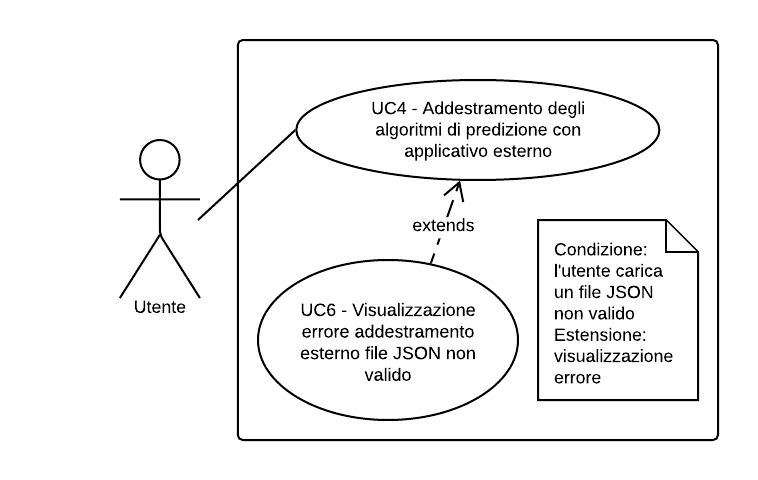
\includegraphics{img/UC4 - Schema generale.png}
%\caption{Schema generale: addestramento degli algoritmi di predizione con applicativo esterno con estensioni}
%\end{figure}
\subsection{UC4 - Addestramento degli algoritmi di predizione con applicativo esterno}
\begin{figure}[H]
	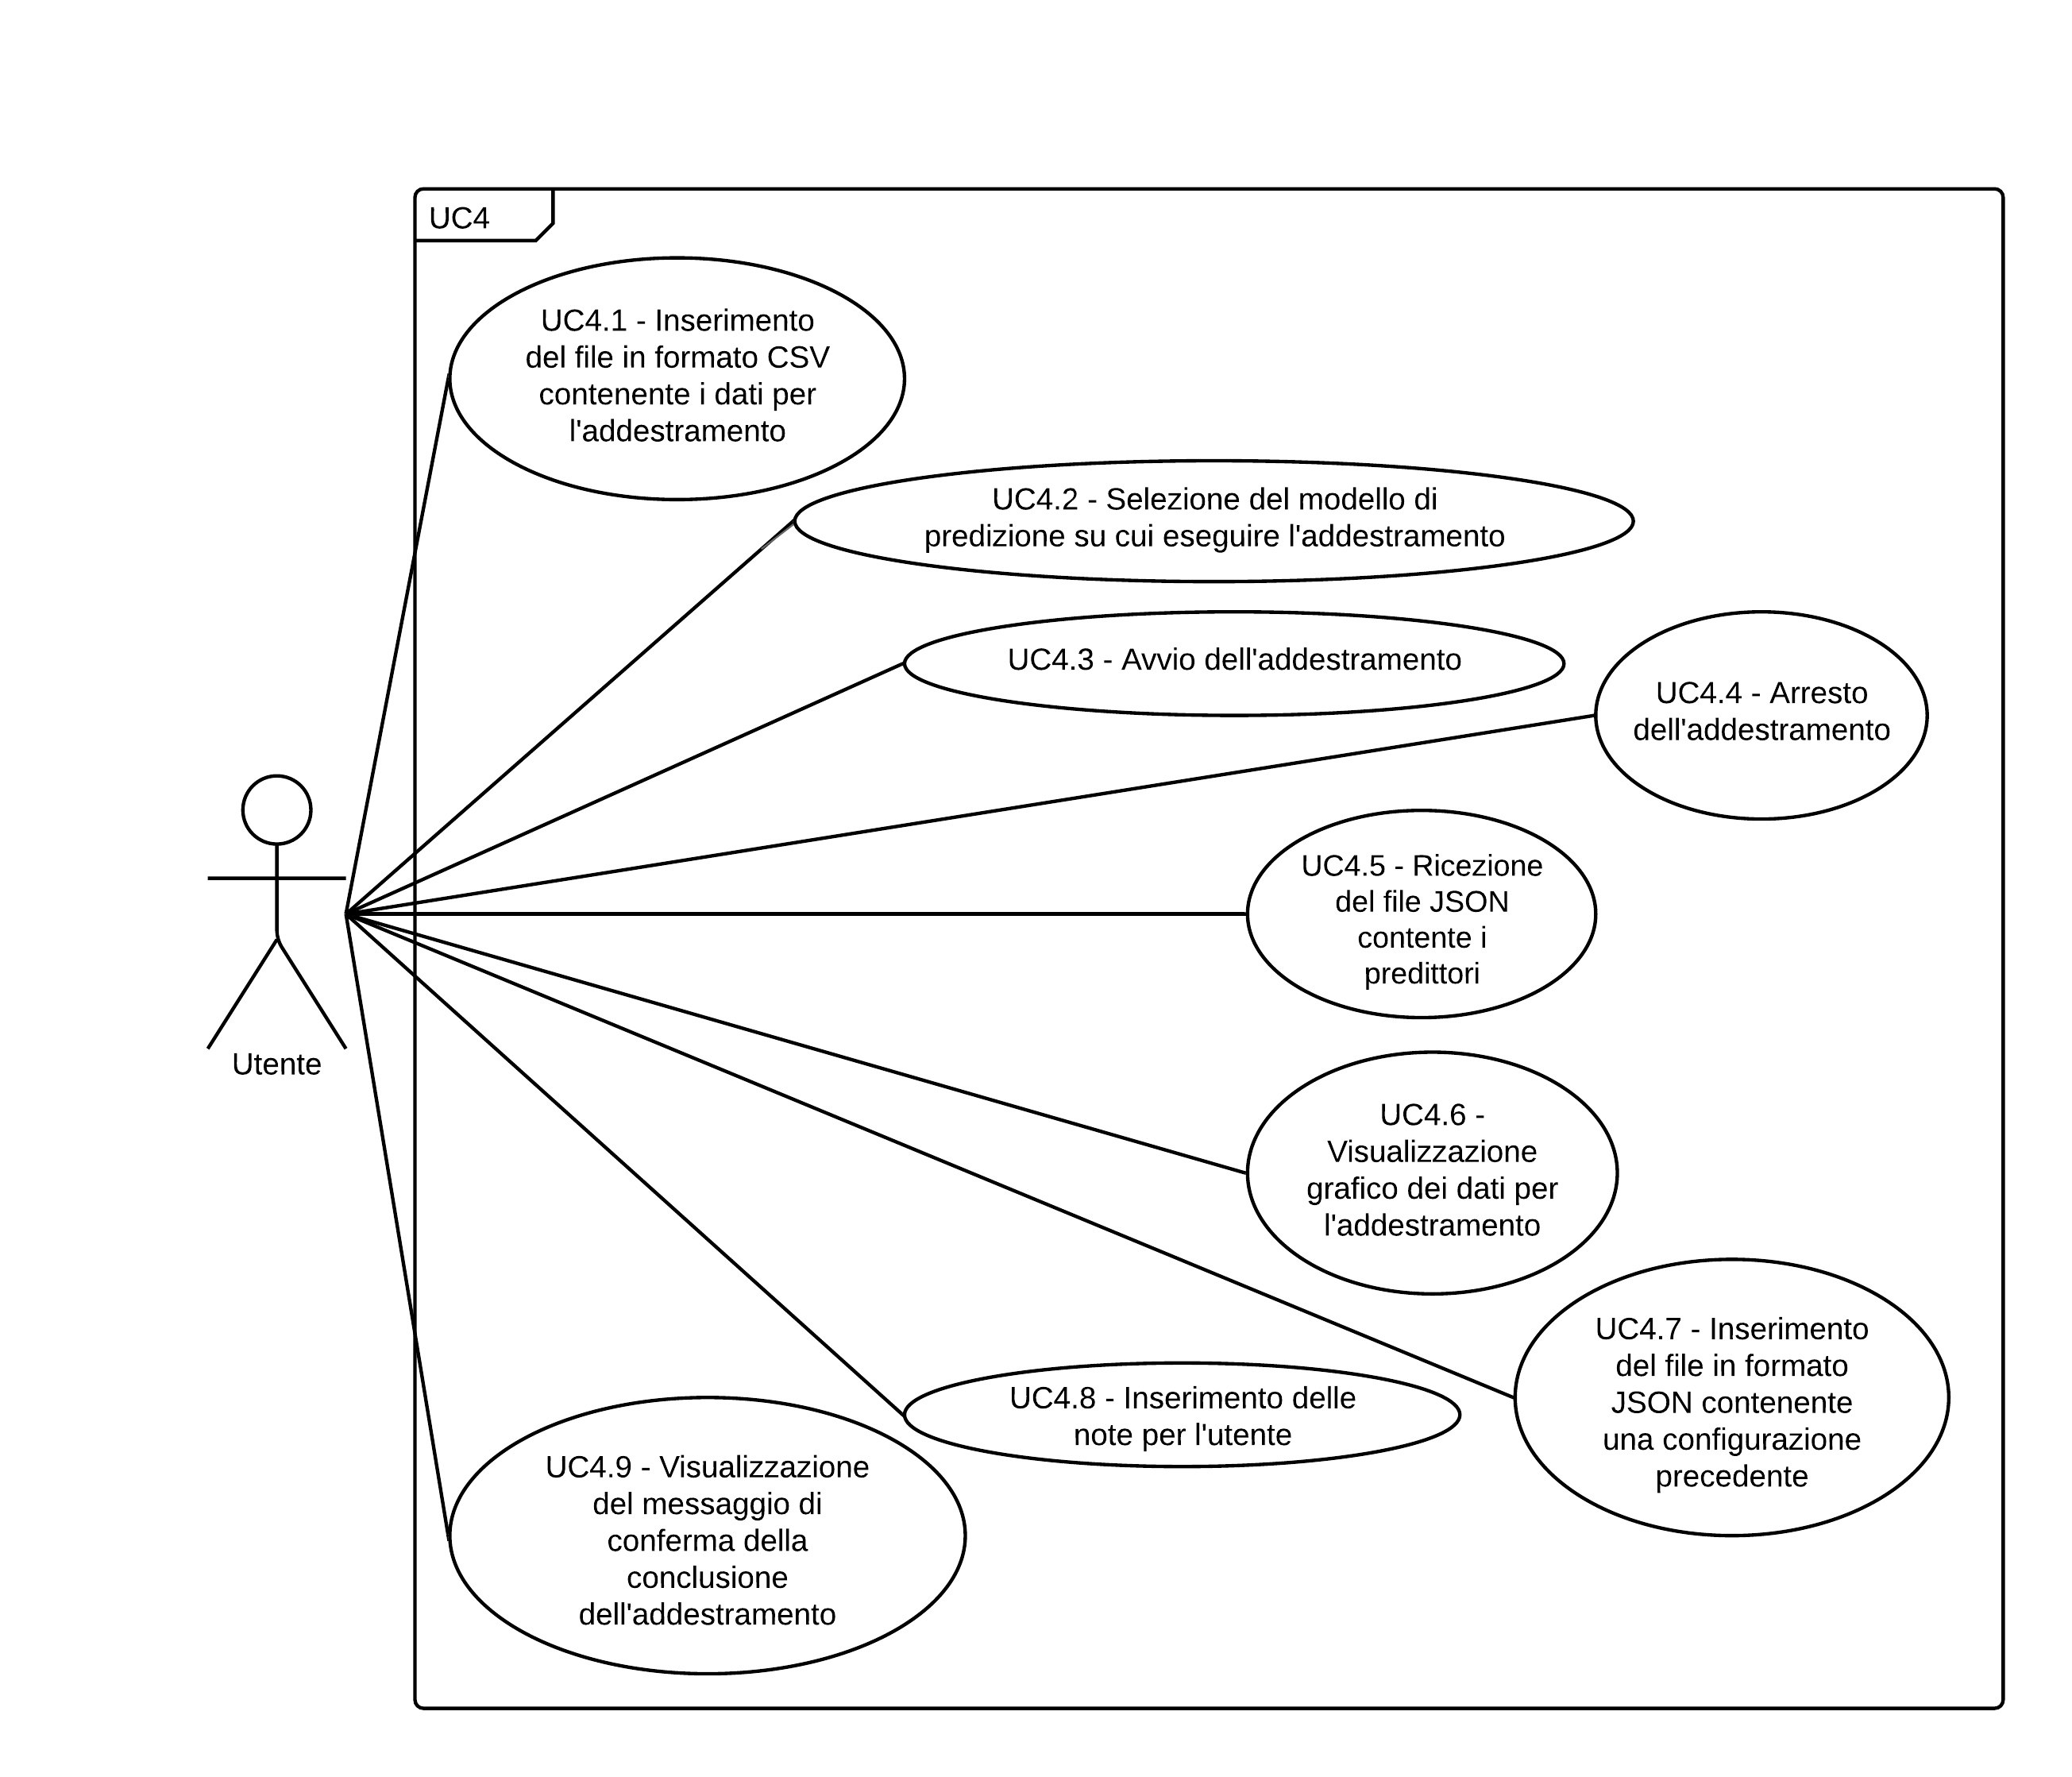
\includegraphics[width=\textwidth,height=\textheight,keepaspectratio]{img/UC4_-_Addestramento_degli_algoritmi_di_predizione_con_applicativo_esterno.png}
	\caption{Diagramma dello use case UC4}
\end{figure}
\begin{itemize}
    \item \textbf{Codice identificativo}: UC4;
    \item \textbf{Titolo}: addestramento degli algoritmi di predizione con applicativo esterno;
    \item \textbf{Attori primari}: utente;
    \item \textbf{Descrizione}: attività di addestramento degli algoritmi di predizione eseguita nell'applicativo esterno a Grafana\glosp utilizzando dei dati inseriti dall'utente;
    \item \textbf{Precondizioni}: l'utente è autenticato nel sistema software Grafana\glo;
    \item \textbf{Postcondizioni}: l'utente ha completato l'addestramento degli algoritmi di predizione;
    \item \textbf{Scenario principale}: 
        \begin{enumerate}
            \item inserimento del file in formato CSV contenente i dati per l'addestramento (UC4.1);
            \item visualizzazione grafico dei dati per l'addestramento (UC4.6);
            \item inserimento del file in formato JSON contenente i dati di una configurazione precedente (UC4.7);
            \item inserimento delle note per l'utente (UC4.8);
            \item selezione del modello di predizione su cui eseguire l'addestramento (UC4.2);
            \item avvio dell'addestramento (UC4.3);
    		\item arresto dell'addestramento (UC4.4);
            \item ricezione del file JSON contenente i predittori (UC4.5);
            \item visualizzazione del messaggio di conferma della conclusione dell'addestramento (UC4.9). 
        \end{enumerate}
    \item \textbf{Estensioni}:
    \begin{enumerate}
    	\item se il caricamento del file CSV non è avvenuto con successo viene visualizzato un messaggio di errore (UC6);
    	\item se il caricamento del file JSON non è avvenuto con successo viene visualizzato un messaggio di errore (UC18).
    \end{enumerate}
\end{itemize}

\subsubsection{UC4.1 - Inserimento del file in formato CSV contenente i dati per l'addestramento}
\begin{itemize}
    \item \textbf{Codice identificativo}: UC4.1;
    \item \textbf{Titolo}: inserimento del file in formato CSV contenente i dati per l'addestramento;
    \item \textbf{Attori primari}: utente;
    \item \textbf{Descrizione}: l'utente inserisce un file in formato CSV contenente i dati per l'addestramento nell'applicazione esterna;
    \item \textbf{Precondizioni}: l'utente è autenticato nel sistema software Grafana\glo;
    \item \textbf{Postcondizioni}: l'utente ha inserito correttamente il file in formato CSV contenente i dati per l'addestramento;
    \item \textbf{Scenario principale}: l'utente inserisce il file in formato CSV contenente i dati per l'addestramento;
\end{itemize}

\subsubsection{UC4.2 - Selezione del modello di predizione su cui eseguire l'addestramento}
\begin{itemize}
	\item \textbf{Codice identificativo}: UC4.2;
	\item \textbf{Titolo}: selezione del modello di predizione su cui eseguire l'addestramento;
	\item \textbf{Attori primari}: utente;
	\item \textbf{Descrizione}: l'utente seleziona il modello di predizione da applicare durante l'addestramento;
	\item \textbf{Precondizioni}: il file CSV contenente i dati per l'addestramento è stato inserito correttamente nell'applicazione esterna;
	\item \textbf{Postcondizioni}: il modello di predizione è stato selezionato correttamente;
	\item \textbf{Scenario principale}: l'utente seleziona un modello di predizione su cui eseguire l'addestramento tra SVM\glosp e RL\glo;
	\item \textbf{Specializzazione}:
	\begin{enumerate}
		\item selezione del modello di predizione SVM\glosp (UC4.10);
		\item selezione del modello di predizione RL\glosp (UC4.11).
	\end{enumerate}   
\end{itemize}

\subsubsection{UC4.3 - Avvio dell'addestramento}
\begin{itemize}
	\item \textbf{Codice identificativo}: UC4.3;
	\item \textbf{Titolo}: avvio dell'addestramento;
	\item \textbf{Attori primari}: utente;
	\item \textbf{Descrizione}: l'utente avvia l'addestramento dell'algoritmo di predizione;
	\item \textbf{Precondizioni}: il file CSV è stato inserito correttamente e il modello di predizione è stato selezionato;
	\item \textbf{Postcondizioni}: l'addestramento è stato avviato con successo;
	\item \textbf{Scenario principale}: l'utente avvia l'addestramento.
\end{itemize}

\subsubsection{UC4.4 - Arresto dell'addestramento}
\begin{itemize}
	\item \textbf{Codice identificativo}: UC4.4;
	\item \textbf{Titolo}: arresto dell'addestramento;
	\item \textbf{Attori primari}: utente;
	\item \textbf{Descrizione}: l'utente arresta l'addestramento prima della sua normale conclusione;
	\item \textbf{Precondizioni}: l'addestramento è stato avviato con successo;
	\item \textbf{Postcondizioni}: l'addestramento è stato arrestato con successo;
	\item \textbf{Scenario principale}: l'utente arresta forzatamente l'addestramento.
\end{itemize}

\subsubsection{UC4.5 - Ricezione del file JSON contente i predittori}
\begin{itemize}
	\item \textbf{Codice identificativo}: UC4.5;
	\item \textbf{Titolo}: ricezione del file JSON contenente i predittori\glo;
	\item \textbf{Attori primari}: utente;
	\item \textbf{Descrizione}: l'applicazione restituisce un file JSON, risultato dal completamento dell'addestramento dei dati, contenente i predittori\glosp per eseguire la predizione;
	\item \textbf{Precondizioni}: l'applicazione esterna ha concluso l'addestramento con successo secondo il suo normale flusso di esecuzione;
	\item \textbf{Postcondizioni}: l'utente ha ricevuto il file JSON, risultato dall'addestramento, contenente i predittori\glosp per eseguire la predizione;
	\item \textbf{Scenario principale}: l'utente riceve il file JSON, risultato dall'addestramento, contenente i predittori\glosp per eseguire la predizione.
\end{itemize}

\subsubsection{UC4.6 - Visualizzazione grafico dei dati per l'addestramento}
\begin{itemize}
	\item \textbf{Codice identificativo}: UC4.6;
	\item \textbf{Titolo}: visualizzazione grafico dei dati per l'addestramento;
	\item \textbf{Attori primari}: utente;
	\item \textbf{Descrizione}: l'utente visualizza il grafico a dispersione rappresentante i dati che ha inserito per l'addestramento;
	\item \textbf{Precondizioni}: il file CSV contenente i dati per l'addestramento è stato inserito correttamente nell'applicazione esterna;
	\item \textbf{Postcondizioni}: l'utente ha visualizzato il grafico a dispersione rappresentante i dati che ha inserito;
	\item \textbf{Scenario principale}: l'utente visualizza il grafico a dispersione rappresentante i dati che ha inserito.
\end{itemize}
\subsubsection{UC4.7 - Inserimento del file in formato JSON contenente una configurazione precedente}
\begin{itemize}
	\item \textbf{Codice identificativo}: UC4.7;
	\item \textbf{Titolo}: inserimento del file in formato JSON contenente una configurazione precedente;
	\item \textbf{Attori primari}: utente;
	\item \textbf{Descrizione}: l'utente inserisce nell'applicazione esterna un file in formato JSON che contiene i dati di una configurazione per addestrare nuovamente l'algoritmo di predizione partendo con una configurazione precedente;
	\item \textbf{Precondizioni}: l'utente è autenticato nel sistema software Grafana\glo;
	\item \textbf{Postcondizioni}: il file in formato JSON contenente una configurazione precedente è stato inserito correttamente;
	\item \textbf{Scenario principale}: l'utente inserisce il file in formato JSON contenente una configurazione precedente.
\end{itemize}
\subsubsection{UC4.8 - Inserimento delle note per l'utente}
\begin{itemize}
	\item \textbf{Codice identificativo}: UC4.8;
	\item \textbf{Titolo}: inserimento delle note per l'utente;
	\item \textbf{Attori primari}: utente;
	\item \textbf{Descrizione}: l'utente inserisce le note che compariranno nel file JSON risultante dall'addestramento dell'algoritmo;
	\item \textbf{Precondizioni}: il file CSV contenente i dati per l'addestramento è stato inserito correttamente nell'applicazione esterna;
	\item \textbf{Postcondizioni}: l'utente ha inserito correttamente le note che compariranno nel file JSON risultante dall'addestramento dell'algoritmo;
	\item \textbf{Scenario principale}: l'utente inserisce le note che compariranno nel file JSON risultante dall'addestramento dell'algoritmo.
\end{itemize}

\subsubsection{UC4.9 - Visualizzazione del messaggio di conferma della conclusione dell'addestramento}
\begin{itemize}
	\item \textbf{Codice identificativo}: UC4.9;
	\item \textbf{Titolo}: visualizzazione del messaggio di conferma della conclusione dell'addestramento;
	\item \textbf{Attori primari}: utente;
	\item \textbf{Descrizione}: l'utente visualizza un messaggio di conferma che l'addestramento è stato concluso ed eseguito correttamente;
	\item \textbf{Precondizioni}: l'addestramento è stato avviato con successo;
	\item \textbf{Postcondizioni}: l'utente ha visualizzato un messaggio di conferma che l'addestramento è stato concluso ed eseguito correttamente;
	\item \textbf{Scenario principale}: l'utente visualizza un messaggio di conferma che l'addestramento è stato concluso ed eseguito correttamente.
\end{itemize}

\subsubsection{UC4.10 - Selezione del modello di predizione SVM}
\begin{itemize}
	\item \textbf{Codice identificativo}: UC4.10;
	\item \textbf{Titolo}: selezione del modello di predizione SVM\glo;
	\item \textbf{Attori primari}: utente;
	\item \textbf{Descrizione}: l'utente seleziona il modello di predizione SVM\glosp da applicare durante l'addestramento nell'applicazione esterna;
	\item \textbf{Precondizioni}: il file CSV contenente i dati per l'addestramento è stato inserito correttamente nell'applicazione esterna;
	\item \textbf{Postcondizioni}: l'utente ha selezionato SVM\glosp come modello di predizione da applicare;
	\item \textbf{Scenario principale}: l'utente seleziona il modello di predizione SVM\glosp su cui eseguire l'addestramento.
\end{itemize}
\subsubsection{UC4.11 - Selezione del modello di predizione RL}
\begin{itemize}
	\item \textbf{Codice identificativo}: UC4.11;
	\item \textbf{Titolo}: selezione del modello di predizione RL\glo;
	\item \textbf{Attori primari}: utente;
	\item \textbf{Descrizione}: l'utente seleziona il modello di predizione RL\glosp da applicare durante l'addestramento nell'applicazione esterna;
	\item \textbf{Precondizioni}: il file CSV contenente i dati per l'addestramento è stato inserito correttamente nell'applicazione esterna;
	\item \textbf{Postcondizioni}: l'utente ha selezionato RL\glosp come modello di predizione da applicare;
	\item \textbf{Scenario principale}: l'utente seleziona il modello di predizione RL\glosp su cui eseguire l'addestramento.
\end{itemize}
\subsubsection{UC4.12 - Selezione del modello di predizione reti neurali}
\begin{itemize}
	\item \textbf{Codice identificativo}: UC4.12;
	\item \textbf{Titolo}: selezione del modello di predizione reti neurali\glo;
	\item \textbf{Attori primari}: utente;
	\item \textbf{Attori secondari}: Grafana\glo;
	\item \textbf{Descrizione}: l'utente seleziona reti neurali\glosp come modello di predizione da applicare durante l'addestramento;
	\item \textbf{Precondizioni}: l'utente è autenticato nel sistema software Grafana\glosp e il file CSV contenente i dati per l'addestramento è stato inserito correttamente;
	\item \textbf{Postcondizioni}: l'utente ha selezionato reti neurali\glosp come modello di predizione da applicare;
	\item \textbf{Scenario principale}: l'utente seleziona il modello di predizione reti neurali\glosp su cui eseguire l'addestramento.
\end{itemize}
\subsubsection{UC4.13 - Selezione del modello di predizione regressioni esponenziali}
\begin{itemize}
	\item \textbf{Codice identificativo}: UC4.13;
	\item \textbf{Titolo}: selezione del modello di predizione regressioni esponenziali;
	\item \textbf{Attori primari}: utente;
	\item \textbf{Attori secondari}: Grafana\glo;
	\item \textbf{Descrizione}: l'utente seleziona regressioni esponenziali come modello di predizione da applicare durante l'addestramento;
	\item \textbf{Precondizioni}: l'utente è autenticato nel sistema software Grafana\glosp e il file CSV contenente i dati per l'addestramento è stato inserito correttamente;
	\item \textbf{Postcondizioni}: l'utente ha selezionato regressioni esponenziali come modello di predizione da applicare;
	\item \textbf{Scenario principale}: l'utente seleziona il modello di predizione regressioni esponenziali su cui eseguire l'addestramento.
\end{itemize}
\subsubsection{UC4.14 - Selezione del modello di predizione regressioni logaritmiche}
\begin{itemize}
	\item \textbf{Codice identificativo}: UC4.14;
	\item \textbf{Titolo}: selezione del modello di predizione regressioni logaritmiche;
	\item \textbf{Attori primari}: utente;
	\item \textbf{Attori secondari}: Grafana\glo;
	\item \textbf{Descrizione}: l'utente seleziona regressioni logaritmiche come modello di predizione da applicare durante l'addestramento;
	\item \textbf{Precondizioni}: l'utente è autenticato nel sistema software Grafana\glosp e il file CSV contenente i dati per l'addestramento è stato inserito correttamente;
	\item \textbf{Postcondizioni}: l'utente ha selezionato regressioni logaritmiche come modello di predizione da applicare;
	\item \textbf{Scenario principale}: l'utente seleziona il modello di predizione regressioni logaritmiche su cui eseguire l'addestramento.
\end{itemize}
\subsubsection{UC4.15 - Selezione del modello di predizione SVM adattata alla Regressione}
\begin{itemize}
	\item \textbf{Codice identificativo}: UC4.15;
	\item \textbf{Titolo}: selezione del modello di predizione SVM\glosp adattata alla Regressione;
	\item \textbf{Attori primari}: utente;
	\item \textbf{Attori secondari}: Grafana\glo;
	\item \textbf{Descrizione}: l'utente seleziona SVM\glosp adattata alla Regressione come modello di predizione da applicare durante l'addestramento;
	\item \textbf{Precondizioni}: l'utente è autenticato nel sistema software Grafana\glosp e il file CSV contenente i dati per l'addestramento è stato inserito correttamente;
	\item \textbf{Postcondizioni}: l'utente ha selezionato SVM\glosp adattata alla Regressione come modello di predizione da applicare;
	\item \textbf{Scenario principale}: l'utente seleziona il modello di predizione SVM\glosp adattata alla Regressione su cui eseguire l'addestramento.
\end{itemize}
	\pagebreak
	\subsection{UC5 - Visualizzazione degli indici di qualità delle previsioni sull'applicativo esterno}
%\begin{figure}[H]
%\includegraphics{img/UC5_-_Visualizzazione_indice_di_qualita_delle_previsioni.png}
%\caption{Diagramma degli use case di UC5}
%\end{figure}
\begin{itemize}
	\item \textbf{Codice identificativo}: UC5;
	\item \textbf{Titolo}: visualizzazione degli indici di qualità delle previsioni;
	\item \textbf{Attori primari}: utente;
	\item \textbf{Descrizione}: l'utente visualizza gli indici numerici che rappresentano la misura di qualità delle previsioni sui dati forniti dall'addestramento;
	\item \textbf{Precondizioni}: l'addestramento è stato eseguito correttamente con l'applicazione esterna;
	\item \textbf{Postcondizioni}: l'utente ha visualizzato gli indici numerici di qualità delle previsioni;
	\item \textbf{Scenario principale}: l'utente visualizza gli indici numerici di qualità delle previsioni.
\end{itemize} 
\subsubsection{UC5.1 - Visualizzazione dell'indice di qualità delle previsioni R$^{2}$}
\begin{itemize}
	\item \textbf{Codice identificativo}: UC5.1;
	\item \textbf{Titolo}: visualizzazione dell'indice di qualità delle previsioni R$^{2}$\glo;
	\item \textbf{Attori primari}: utente;
	\item \textbf{Descrizione}: l'utente visualizza l'indice numerico che rappresenta la misura di qualità delle previsioni sui dati forniti attraverso il meccanismo R$^{2}$\glo;
	\item \textbf{Precondizioni}: l'addestramento è stato eseguito con l'applicazione esterna;
	\item \textbf{Postcondizioni}: l'utente ha visualizzato l'indice di qualità delle previsioni R$^{2}$\glo;
	\item \textbf{Scenario principale}: l'utente visualizza l'indice di qualità delle previsioni R$^{2}$\glo.
\end{itemize} 
\subsubsection{UC5.2 - Visualizzazione degli indici di qualità delle previsioni Precision}
\begin{itemize}
	\item \textbf{Codice identificativo}: UC5.2;
	\item \textbf{Titolo}: visualizzazione degli indici di qualità delle previsioni Precision\glo;
	\item \textbf{Attori primari}: utente;
	\item \textbf{Descrizione}: l'utente visualizza l'indice numerico che rappresenta la misura di qualità delle previsioni sui dati forniti attraverso il meccanismo Precision\glo;
	\item \textbf{Precondizioni}: l'addestramento è stato eseguito con l'applicazione esterna;
	\item \textbf{Postcondizioni}: l'utente ha visualizzato l'indice di qualità delle previsioni Precision\glo;
	\item \textbf{Scenario principale}: l'utente visualizza l'indici di qualità delle previsioni Precision\glo.
\end{itemize} 
\subsubsection{UC5.3 - Visualizzazione degli indici di qualità delle previsioni Recall}
\begin{itemize}
	\item \textbf{Codice identificativo}: UC5.3;
	\item \textbf{Titolo}: visualizzazione degli indici di qualità delle previsioni Recall\glo;
	\item \textbf{Attori primari}: utente;
	\item \textbf{Descrizione}: l'utente visualizza l'indice numerico che rappresenta la misura di qualità delle previsioni sui dati forniti attraverso il meccanismo Recall\glo;
	\item \textbf{Precondizioni}: l'addestramento è stato eseguito con l'applicazione esterna;
	\item \textbf{Postcondizioni}: l'utente ha visualizzato l'indici di qualità delle previsioni Recall\glo;
	\item \textbf{Scenario principale}: l'utente visualizza l'indici di qualità delle previsioni Recall\glo.
\end{itemize} 

	\pagebreak
	\subsection{UC6 - Visualizzazione errore addestramento esterno file CSV non valido}
\begin{itemize}
	\item \textbf{Codice identificativo}: UC6;
	\item \textbf{Titolo}: visualizzazione errore addestramento esterno file CSV non valido;
	\item \textbf{Attori primari}: utente;
	\item \textbf{Descrizione}:  l'utente visualizza un errore relativo al caricamento di un file CSV contenente i dati per l'addestramento non valido;
	\item \textbf{Precondizioni}: l'utente carica un file CSV non valido;
	\item \textbf{Postcondizioni}: l'utente ha visualizzato l'errore file CSV non valido;	
	\item \textbf{Scenario principale}: l'utente visualizza il messaggio di errore causato dall'inserimento di un file JSON non valido.	
\end{itemize}

	\pagebreak
	\subsection{UC19 - Abilitazione del plug-in}
\begin{figure}[H]
	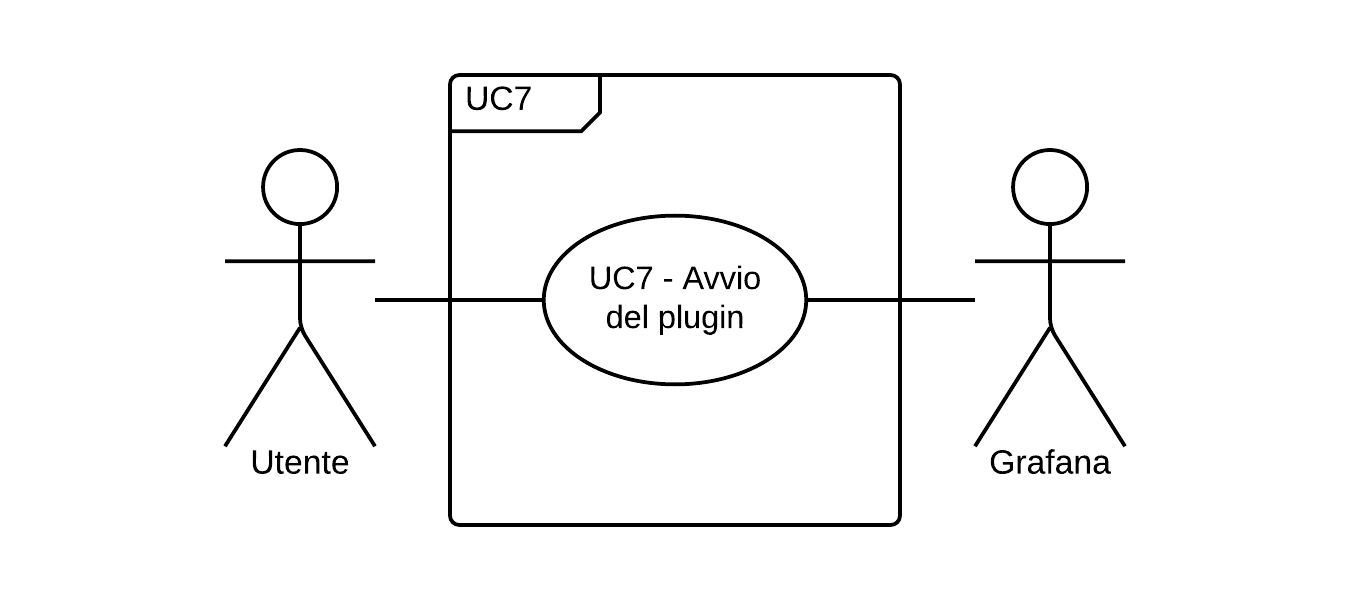
\includegraphics{img/UC7_-_Avvio_plugin.png}
	\caption{Diagramma degli use case di UC7}
\end{figure}
\begin{itemize}
	\item \textbf{Codice identificativo}: UC19;
	\item \textbf{Titolo}: abilitazione del plug-in;
	\item \textbf{Attori primari}: utente;
	\item \textbf{Attori secondari}: Grafana\glo;
	\item \textbf{Descrizione}: l'utente esegue l'attività di abilitazione del plug-in dalle impostazioni di Grafana\glo;
	\item \textbf{Precondizioni}: l'utente è autenticato nel sistema software Grafana\glo;
	\item \textbf{Postcondizioni}: il plug-in è stato abilitato correttamente;
	\item \textbf{Scenario principale}: l'utente accede alle impostazioni di Grafana\glosp ed abilita il plug-in. In questo modo esso viene abilitato e sarà possibile utilizzarlo aggiungendo il suo pannello alle dashboard\glosp di Grafana\glo.
\end{itemize}

\subsection{UC7 - Avvio del plug-in}
\begin{figure}[H]
	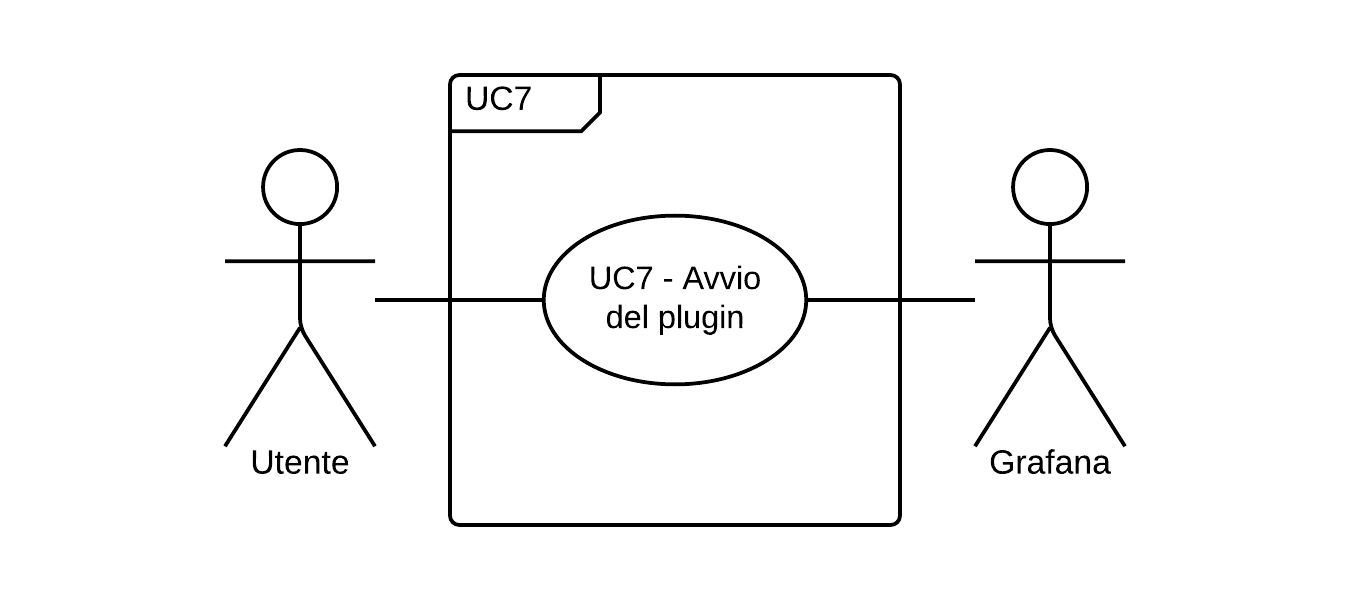
\includegraphics{img/UC7_-_Avvio_plugin.png}
	\caption{Diagramma degli use case di UC7}
\end{figure}
\begin{itemize}
	\item \textbf{Codice identificativo}: UC7;
	\item \textbf{Titolo}: avvio del plug-in;
	\item \textbf{Attori primari}: utente;
	\item \textbf{Attori secondari}: Grafana\glo;
	\item \textbf{Descrizione}: l'utente esegue l'attività di avvio del plug-in che consiste nel collegamento del pannello da esso fornito ad una dashboard\glosp configurata dall'utente;
	\item \textbf{Precondizioni}: l'utente è autenticato nel sistema software Grafana\glo, ha abilitato il plug-in ed ha creato e configurato una dashboard\glosp per la visualizzazione del risultato;
	\item \textbf{Postcondizioni}: il plug-in è stato avviato correttamente;
	\item \textbf{Scenario principale}: l'utente accede alla dashboard\glosp e collega il pannello fornito dal plug-in. In questo modo esso viene avviato.
\end{itemize}

	\pagebreak
	\subsection{UC8 - Caricamento file JSON di addestramento}
\begin{figure}[H]
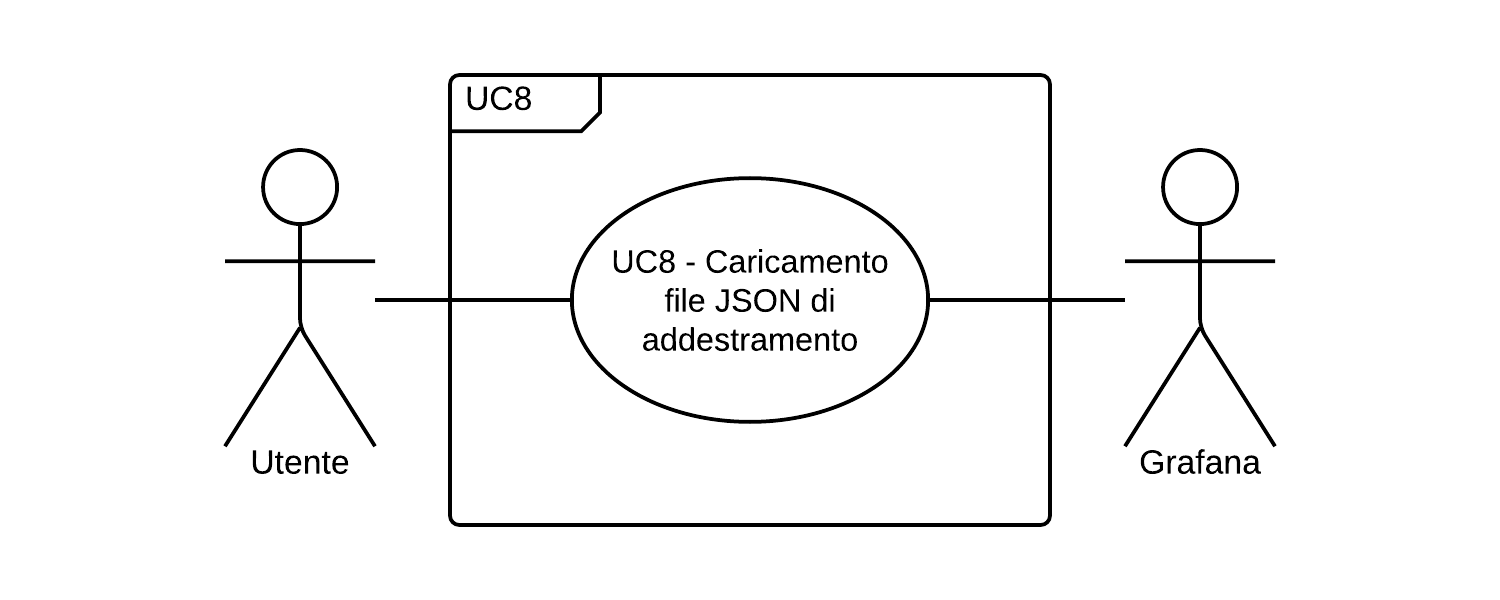
\includegraphics{img/UC8_-_Caricamento_file_JSON_di_addestramento.png}
\caption{Diagramma degli use case di UC8}
\end{figure}
\begin{itemize}
	\item \textbf{Codice identificativo}: UC8;
	\item \textbf{Titolo}: Caricamento file JSON di addestramento;
	\item \textbf{Attori primari}: Utente;
	\item \textbf{Attori secondari}: Grafana\glo;
	\item \textbf{Descrizione}: L'utente esegue l'attività di caricamento del file JSON contenente i dati di addestramento da utilizzare durante la previsione;
	\item \textbf{Precondizioni}: L'utente è autenticato nel sistema software Grafana\glosp, ha configurato una dashboard\glosp per la visualizzazione del risultato e ha avviato il plugin;
	\item \textbf{Postcondizioni}: Il file JSON contenente i dati di addestramento è stato caricato correttamente;
	\item \textbf{Scenario principale}: L'utente carica il file JSON di addestramento.
\end{itemize}
	\pagebreak
	%\subsection{Schema generale: associazione dei nodi al flusso dati con estensioni}
%\begin{figure}[H]
%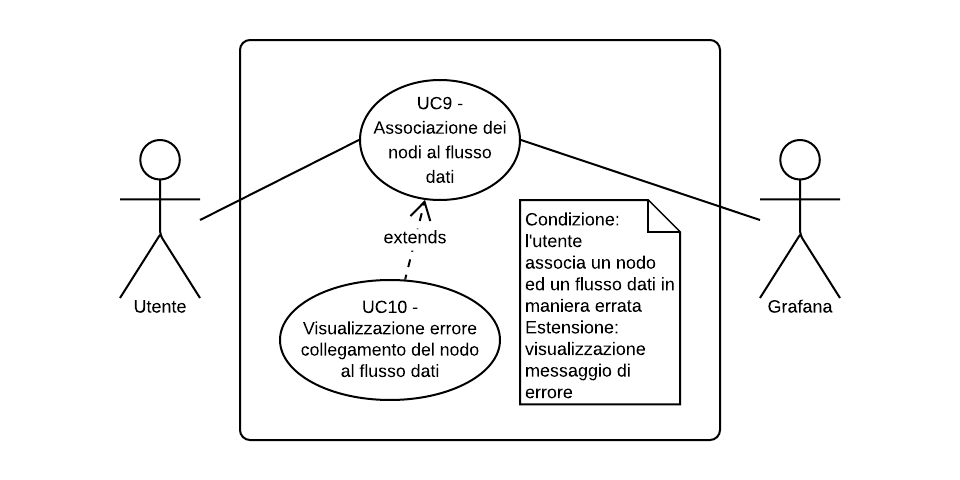
\includegraphics{img/UC9 - Schema generale.png}
%\caption{Schema generale: associazione dei nodi al flusso dati con estensioni}
%\end{figure}
\subsection{UC9 - Associazione dei predittori al flusso dati}
\begin{figure}[H]
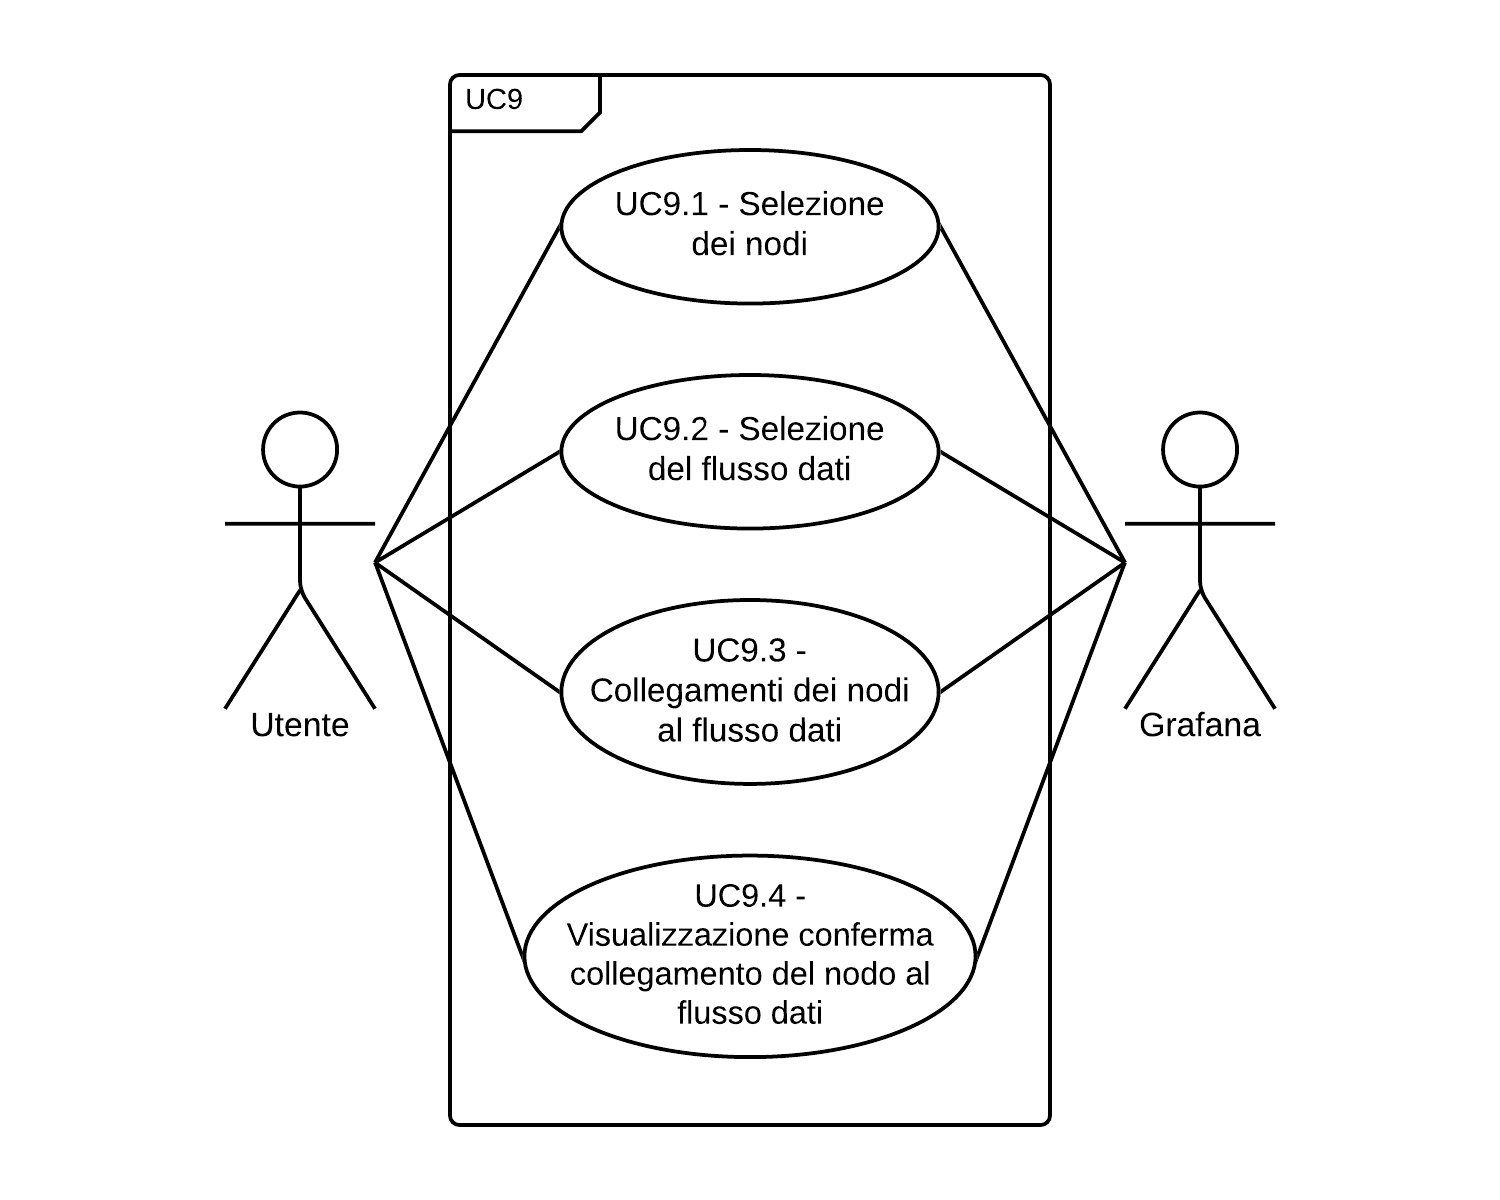
\includegraphics{img/UC9_-_Associazione_dei_nodi_al_flusso_dati.png}
\caption{Diagramma degli use case di UC9}
\end{figure}
\begin{itemize}
	\item \textbf{Codice identificativo}: UC9;
	\item \textbf{Titolo}: associazione dei predittori al flusso dati;
	\item \textbf{Attori primari}: utente;
	\item \textbf{Attori secondari}: Grafana\glo;
	\item \textbf{Descrizione}: l'utente esegue l'associazione dei predittori individuati per l'attività di previsione;
	\item \textbf{Precondizioni}: l'utente è autenticato nel sistema software Grafana\glosp, ha avviato il plug-in e ha caricato il file JSON con i dati di addestramento;
	\item \textbf{Postcondizioni}: i predittori sono stati associati al flusso dati con successo;
	\item \textbf{Scenario principale}: 
		\begin{itemize}
			\item selezione del predittore (UC9.1);
			\item selezione del flusso dati (UC9.2);
			\item collegamenti del predittore al flusso dati (UC9.3);
			\item visualizzazione conferma collegamento del predittore al flusso dati (UC9.4).
		\end{itemize}
	\item \textbf{Estensioni}:
		\begin{itemize}
			\item se l'utente crea un abbinamento non valido tra un predittore ed il flusso dati viene visualizzato un messaggio di errore (UC10).
		\end{itemize}
\end{itemize}

\subsubsection{UC9.1 - Selezione del predittore}
\begin{itemize}
	\item \textbf{Codice identificativo}: UC9.1;
	\item \textbf{Titolo}: selezioni dei predittori;
	\item \textbf{Attori primari}: utente;
	\item \textbf{Attori secondari}: Grafana\glo;
	\item \textbf{Descrizione}: l'utente seleziona il predittore tramite il plug-in;
	\item \textbf{Precondizioni}: l'utente ha avviato correttamente il plug-in;
	\item \textbf{Postcondizioni}: l'utente ha selezionato correttamente il predittore;
	\item \textbf{Scenario principale}: l'utente seleziona il predittore da associare al flusso di dati.
\end{itemize}

\subsubsection{UC9.2 - Selezione del flusso dati}
\begin{itemize}
	\item \textbf{Codice identificativo}: UC9.2;
	\item \textbf{Titolo}: selezione del flusso dati;
	\item \textbf{Attori primari}: utente;
	\item \textbf{Attori secondari}: Grafana\glo;
	\item \textbf{Descrizione}: l'utente seleziona il flusso di dati tramite il plug-in;
	\item \textbf{Precondizioni}: l'utente ha avviato correttamente il plug-in;
	\item \textbf{Postcondizioni}: l'utente ha selezionato correttamente flusso dati;
	\item \textbf{Scenario principale}: l'utente seleziona il flusso dati a cui viene associato il predittore.
\end{itemize}

\subsubsection{UC9.3 - Collegamenti del predittore al flusso dati}
\begin{itemize}
	\item \textbf{Codice identificativo}: UC9.3;
	\item \textbf{Titolo}: collegamenti del predittore al flusso dati;
	\item \textbf{Attori primari}: utente;
	\item \textbf{Attori secondari}: Grafana\glo;
	\item \textbf{Descrizione}: l'utente esegue il collegamento del predittore al flusso dati;
	\item \textbf{Precondizioni}: l'utente ha avviato correttamente il plug-in, ha selezionato il predittore ed il flusso dati;
	\item \textbf{Postcondizioni}: l'utente ha collegato correttamente il predittore al flusso dati;
	\item \textbf{Scenario principale}: l'utente seleziona il flusso dati a cui viene associato il predittore.
\end{itemize}

\subsubsection{UC9.4 - Visualizzazione conferma collegamento del predittore al flusso dati}
\begin{itemize}
	\item \textbf{Codice identificativo}: UC9.4;
	\item \textbf{Titolo}: visualizzazione conferma collegamento del predittore al flusso dati;
	\item \textbf{Attori primari}: utente;
	\item \textbf{Attori secondari}: Grafana\glo;
	\item \textbf{Descrizione}: l'utente visualizza la conferma di collegamento del predittore al flusso dati avvenuta con successo;
	\item \textbf{Precondizioni}: l'utente ha avviato il plug-in e ha eseguito il collegamento del predittore al flusso dati;
	\item \textbf{Postcondizioni}: l'utente ha visualizzato la conferma del collegamento del predittore al flusso dati;
	\item \textbf{Scenario principale}: l'utente visualizza la conferma del collegamento del predittore al flusso dati.
\end{itemize}
	\pagebreak
	\section{UC10 - Visualizzazione errore collegamento del nodo al flusso dati}
\begin{itemize}
    \item \textbf{Codice identificativo}: UC10;
    \item \textbf{Titolo}: Visualizzazione errore collegamento del nodo al flusso dati;
    \item \textbf{Attori primari}: Utente;
    \item \textbf{Attori secondari}: Grafana\glo;
    \item \textbf{Descrizione}: l'utente visualizza il messaggio di errore causato da un collegamento tra un nodo e il flusso dati non valido;
    \item \textbf{Precondizioni}: l'utente deve aver effettuato il login nella piattaforma Grafana\glo e ha associato tra loro un nodo e il flusso dati in maniera errata;
    \item \textbf{Postcondizioni}: l'utente visualizza il messaggio di errore causato da un abbinamento non valido tra un nodo e il flusso dati;
    \item \textbf{Scenario principale}: l'utente visualizza il messaggio di errore causato da un collegamento non valido tra un nodo e il flusso dati.
\end{itemize}
	\pagebreak
	%\section{UC11 - Visualizzazione dei risultati della previsione}
\begin{itemize}
    \item \textbf{Codice identificativo}: UC11;
    \item \textbf{Titolo}: Visualizzazione dei risultati della previsione;
    \item \textbf{Attori primari}: Utente;
    \item \textbf{Attori secondari}: Grafana\glo;
    \item \textbf{Descrizione}: l'utente visualizza un grafico che riporta il risultato della previsione effettuata sul flusso dati;
    \item \textbf{Precondizioni}: l'utente deve aver effettuato il login nella piattaforma Grafana\glo, avviato il plugin, inserito il JSON per l'addestramento del modello e associato i nodi al flusso dati in maniera corretta;
    \item \textbf{Postcondizioni}: l'utente visualizza un grafico che riporta il risultato della previsione effettuata sul flusso dati;
    \item \textbf{Scenario principale}: l'utente visualizza un grafico che riporta il risultato della previsione effettuata sul flusso dati.
\end{itemize}
	%\pagebreak
	\section{UC12 - Rimozione plugin}
\begin{itemize}
    \item \textbf{Codice identificativo}: UC12;
    \item \textbf{Titolo}: Rimozione plugin;
    \item \textbf{Attori primari}: Utente;
    \item \textbf{Attori secondari}: Grafana\glo;
    \item \textbf{Descrizione}: l'utente rimuove il pannello di Grafana\glosp dove è inserito il plugin provocandone quindi la rimozione;
    \item \textbf{Precondizioni}: l'utente deve aver effettuato il login nella piattaforma Grafana\glo e avviato il plugin;
    \item \textbf{Postcondizioni}: l'utente ha rimosso con successo il plugin da Grafana\glo;
    \item \textbf{Scenario principale}: l'utente rimuove il pannello di Grafana\glosp in cui è inserito il plugin provocandone quindi la rimozione.
\end{itemize}
	\pagebreak
	\subsection{Schema generale UC13}
\begin{figure}[H]
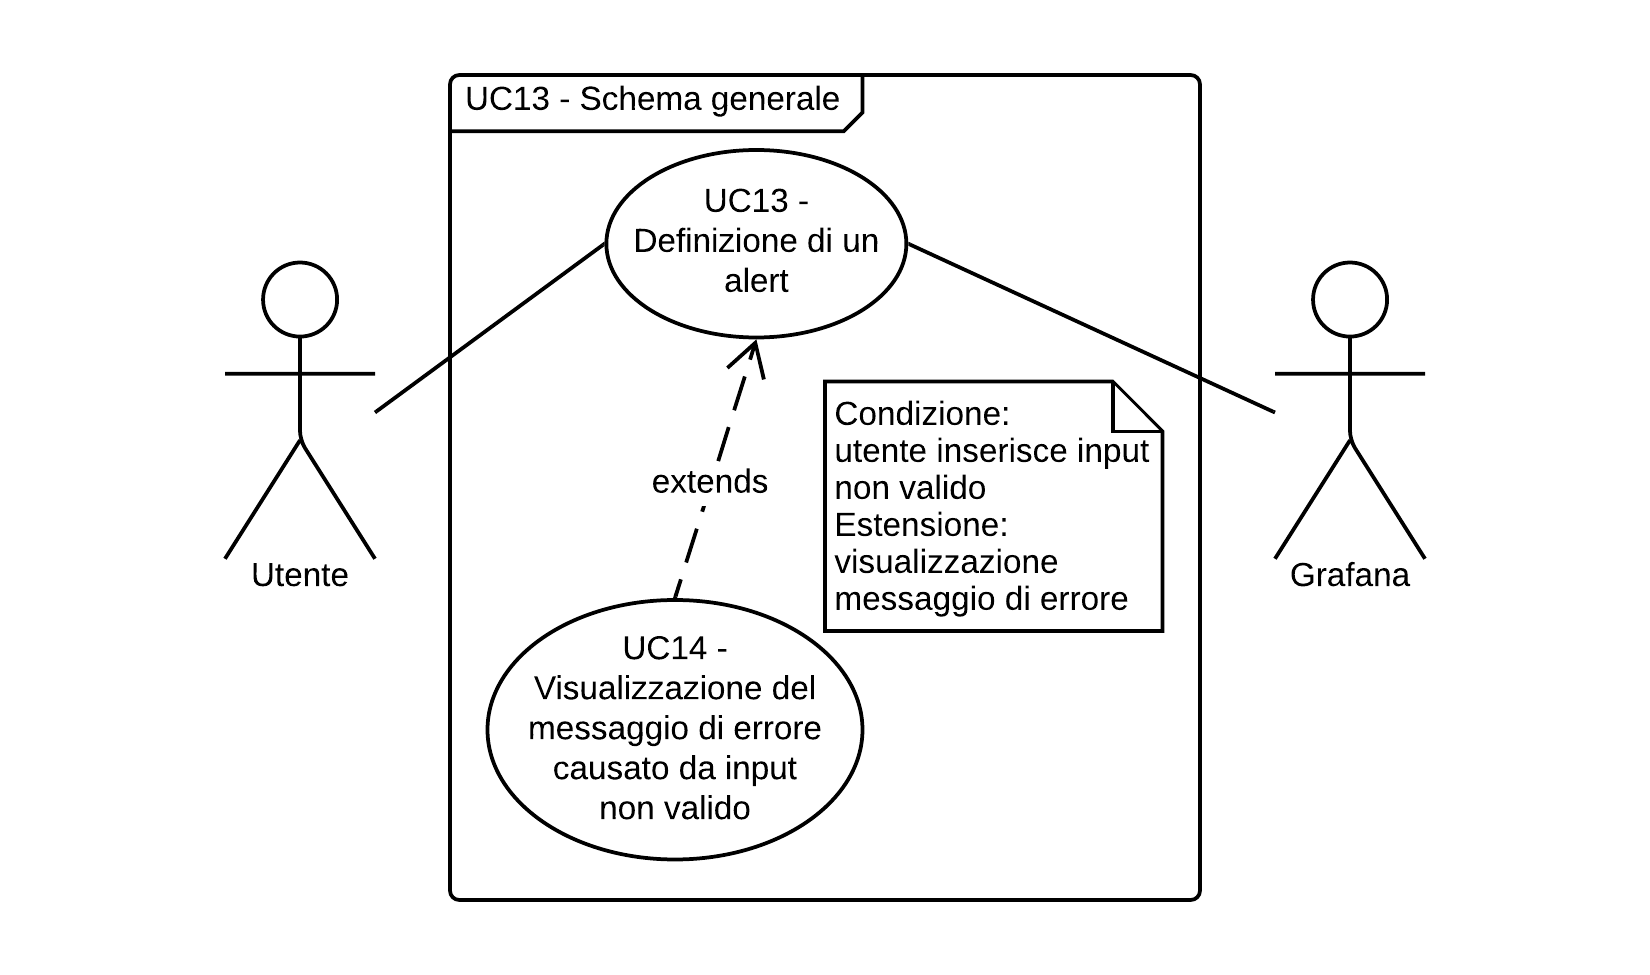
\includegraphics{img/UC13_-_Schema_generale.png}
\caption{Schema generale UC13}
\end{figure}
\subsection{UC13 - Definizione di un alert}
\begin{figure}[H]
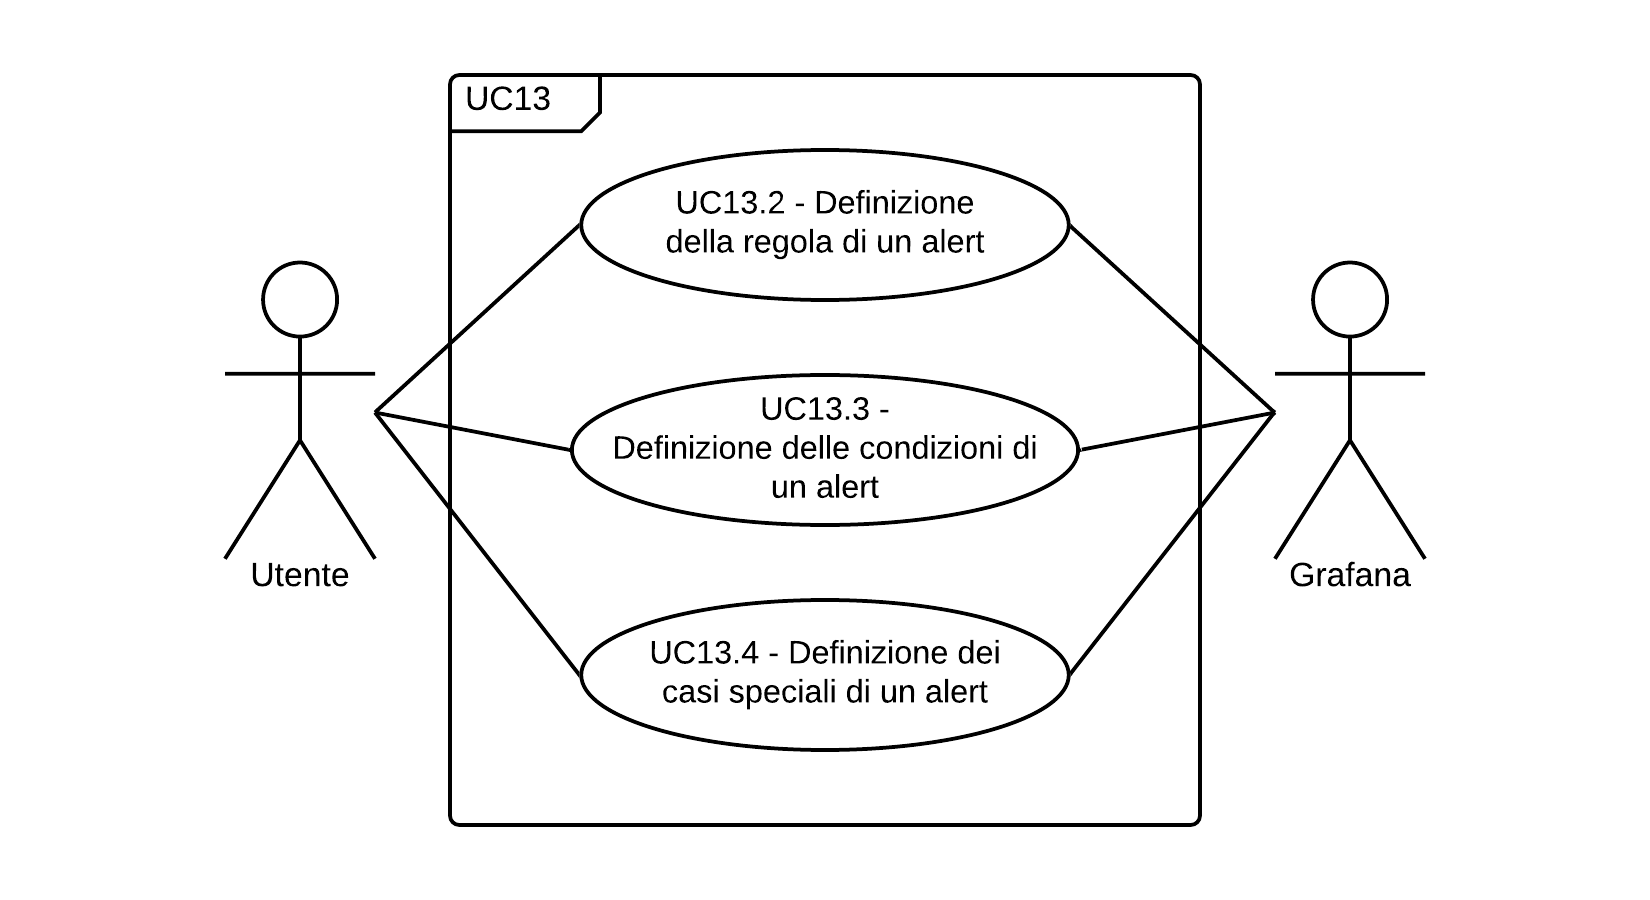
\includegraphics{img/UC13_-_Definizione_di_un_alert.png}
\caption{Diagramma degli use case di UC13}
\end{figure}
\begin{itemize}
	\item \textbf{Codice identificativo}: UC13;
	\item \textbf{Titolo}: Definizione di un alert\glo;
	\item \textbf{Attore primario}: Utente;
	\item \textbf{Attore secondario}: Grafana\glo;
	\item \textbf{Descrizione}: Questo caso d'uso descrive la funzionalità offerta da Grafana\glosp di definire alert\glosp sulle serie di dati che monitora;
	\item \textbf{Precondizione}: L'utente è autenticato nel sistema software Grafana\glosp ed è presente una istanza di Grafana\glosp cloud o locale su cui è stato aggiunto un pannello grafico che monitora una serie di dati;
	\item \textbf{Postcondizione}: Viene inserito e definito con successo un alert\glosp nel pannello grafico scelto;
	\item \textbf{Scenario principale}: 
	\begin{enumerate}
		\item Inserimento di un alert\glosp (UC13.1);
		\item Definizione della regola dell'alert\glosp (UC13.2);
		\item Definizione delle condizioni dell'alert\glosp (UC13.3);
		\item Definizione dei casi speciali dell'alert\glosp (UC13.4).
	\end{enumerate}

	\item \textbf{Estensioni}:	
	\begin{enumerate}
		\item Visualizzazione del messaggio di errore causato da input non valido (UC13).
	\end{enumerate}
\end{itemize}

\subsubsection{UC13.1 - Inserimento di un alert}
\begin{itemize}
	\item \textbf{Codice identificativo}: UC13.1;
	\item \textbf{Titolo}: Inserimento di un alert\glo;
	\item \textbf{Attore primario}: Utente;
	\item \textbf{Attore secondario}: Grafana\glo;
	\item \textbf{Descrizione}: Grafana\glosp fornisce all'utente un modo per inserire alert\glosp sui pannelli grafici;
	\item \textbf{Precondizione}: L'utente deve aver inserito in una dashboard\glosp un pannello grafico;
	\item \textbf{Postcondizione}: Il pannello grafico possiede ora un alert\glo;
	\item \textbf{Scenario principale}: L'utente inserisce in un pannello grafico un alert\glo.
\end{itemize}

\subsubsection{UC13.2 - Definizione della regola di un alert}
\begin{itemize}
	\item \textbf{Codice identificativo}: UC13.2;
	\item \textbf{Titolo}: Definizione della regola dell'alert\glo;
	\item \textbf{Attore primario}: Utente;
	\item \textbf{Attore secondario}: Grafana\glo;
	\item \textbf{Descrizione}: Dopo aver aggiunto un alert\glosp ad un pannello grafico l'utente ha la possibilità di definire la sua regola principale di funzionamento;
	\item \textbf{Precondizione}: L'utente ha aggiunto un alert\glosp al pannello grafico;
	\item \textbf{Postcondizione}: L'utente tramite le funzioni offerte da Grafana\glosp ha definito la regola dell'alert\glosp precedentemente aggiunto;
	\item \textbf{Scenario principale}: L'utente definisce le regole di funzionamento dell'alert\glosp appena inserito, usando le funzioni previste da Grafana\glosp ed inserendo quindi nome e tempi di interrogazione.
\end{itemize}

\subsubsection{UC13.3 - Definizione delle condizioni di un alert}
\begin{itemize}
	\item \textbf{Codice identificativo}: UC13.3;
	\item \textbf{Titolo}: Definizione delle condizioni dell'alert\glo;
	\item \textbf{Attore primario}: Utente;
	\item \textbf{Attore secondario}: Grafana\glo;
	\item \textbf{Descrizione}: Dopo aver aggiunto un alert\glosp ad un pannello grafico l'utente ha la possibilità di definire le sue condizioni di funzionamento;
	\item \textbf{Precondizione}: L'utente ha aggiunto un alert\glosp al pannello grafico;
	\item \textbf{Postcondizione}: L'utente tramite le funzioni offerte da Grafana\glosp ha definito una o più condizioni dell'alert\glosp precedentemente aggiunto;
	\item \textbf{Scenario principale}: L'utente definisce la condizioni di funzionamento dell'alert\glosp appena inserito, usando le funzioni previste da Grafana\glosp e selezionando quindi la funzione di aggregazione dati ed il valore soglia che attiva l'allarme.
\end{itemize}

\subsubsection{UC13.4 - Definizione dei casi speciali di un alert}
	\begin{itemize}
	\item \textbf{Codice identificativo}: UC13.4;
	\item \textbf{Titolo}: Definizione dei casi speciali dell'alert\glo;
	\item \textbf{Attore primario}: Utente;
	\item \textbf{Attore secondario}: Grafana\glo;
	\item \textbf{Descrizione}: Dopo aver aggiunto un alert\glosp ad un pannello grafico l'utente ha la possibilità di definire il suo comportamento al verificarsi di casi particolari;
	\item \textbf{Precondizione}: L'utente ha aggiunto un alert\glosp al pannello grafico;
	\item \textbf{Postcondizione}: L'utente, tramite le funzioni offerte da Grafana\glosp, ha definito uno o più comportamenti speciali dell'alert\glosp precedentemente aggiunto;
	\item \textbf{Scenario principale}: L'utente definisce i comportamenti speciali dell'alert\glosp nei casi particolari come assenza di dati o errori di esecuzione. Per farlo utilizza le funzioni previste da Grafana\glosp selezionando quindi i comportamenti desiderati.
\end{itemize} 
	\pagebreak
	\subsection{UC14 - Visualizzazione del messaggio di errore causato da input non valido}
\begin{itemize}
	\item \textbf{Codice identificativo}: UC14;
	\item \textbf{Titolo}: visualizzazione del messaggio di errore causato da input non valido;
	\item \textbf{Attori primari}: utente;
	\item \textbf{Attori secondari}: Grafana\glo;
	\item \textbf{Descrizione}: l'utente visualizza il messaggio di errore causato da input non valido;
	\item \textbf{Precondizioni}: l'utente è autenticato nel sistema software Grafana\glosp ed ha inserito un alert\glosp su cui ha compilato un campo numerico inserendo solo lettere o lasciandolo vuoto;
	\item \textbf{Postcondizioni}: l'utente visualizza il messaggio di errore causato da input non valido;
	\item \textbf{Scenario principale}: l'utente visualizza il messaggio di errore causato da input non valido.
\end{itemize}
	\pagebreak
	\subsection{UC15 - Sospensione di un alert}
\begin{figure}[H]
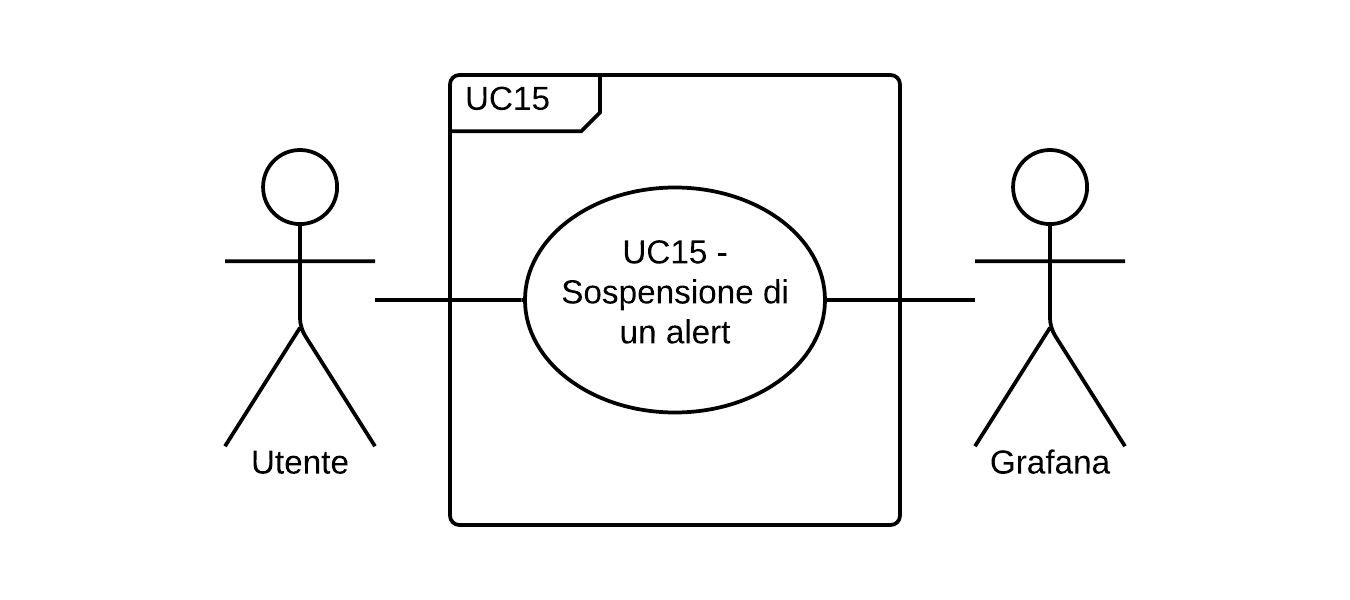
\includegraphics{img/UC15_-_Sospensione_di_un_alert.png}
\caption{Diagramma degli use case di UC15}
\end{figure}
\begin{itemize}
	\item \textbf{Codice identificativo}: UC15;
	\item \textbf{Titolo}: Sospensione di un alert\glo;
	\item \textbf{Attore primario}: Utente;
	\item \textbf{Attore secondario}: Grafana\glo;
	\item \textbf{Descrizione}: L'utente esegue la sospensione di un alert\glosp, bloccandone temporaneamente l'esecuzione;
	\item \textbf{Precondizione}: L'utente è autenticato nel sistema software Grafana\glosp ed ha aperto il pannello di visualizzazione alert\glo;
	\item \textbf{Postcondizione}: L'alert\glosp selezionato dall'utente è sospeso;
	\item \textbf{Scenario principale}: Utilizzando l'apposita funzione offerta da Grafana\glosp l'utente sospende l'esecuzione dell'alert\glosp che ha selezionato.
\end{itemize} 

	\pagebreak
	\subsection{UC16 - Rimozione di un alert}
\begin{figure}[H]
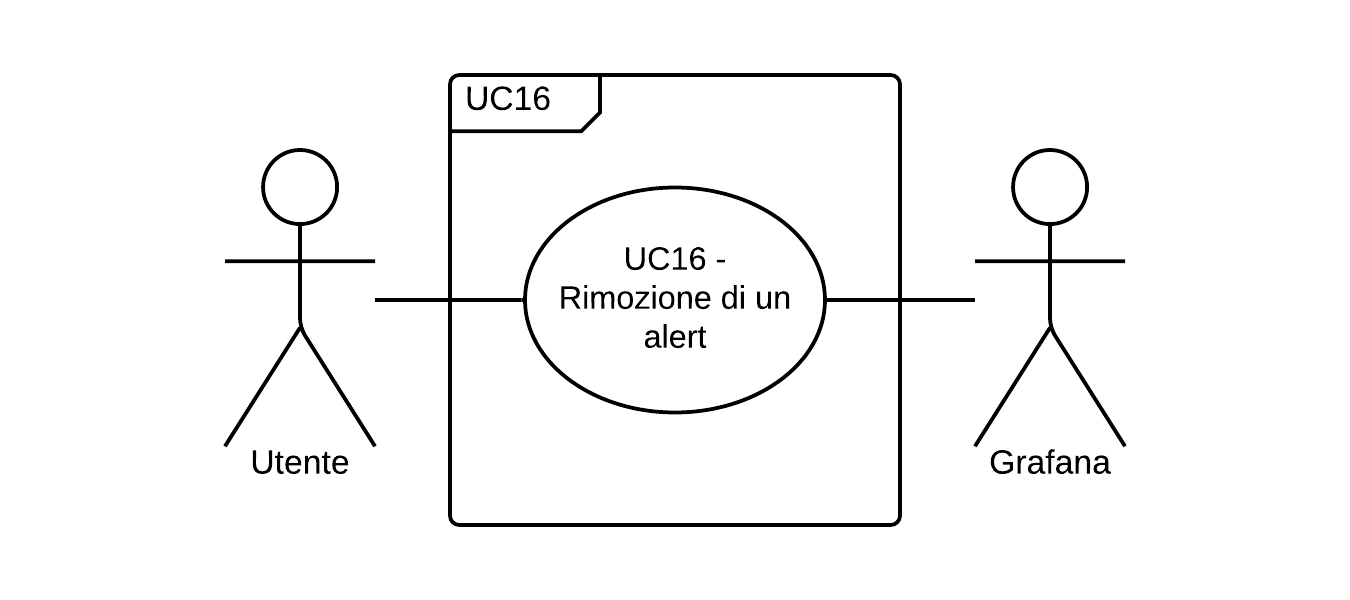
\includegraphics{img/UC16_-_Rimozione_di_un_alert.png}
\caption{Diagramma degli use case di UC16}
\end{figure}
\begin{itemize}
	\item \textbf{Codice identificativo}: UC16;
	\item \textbf{Titolo}: Rimozione di un alert\glo;
	\item \textbf{Attore primario}: Utente;
	\item \textbf{Attore secondario}: Grafana\glo;
	\item \textbf{Descrizione}: L'utente rimuove un alert\glosp da un pannello grafico;
	\item \textbf{Precondizione}: L'utente è autenticato nel sistema software Grafana\glosp ed ha inserito e selezionato almeno un alert\glo;
	\item \textbf{Postcondizione}: L'alert\glosp selezionato dall'utente è eliminato;
	\item \textbf{Scenario principale}: Utilizzando l'apposita funzione offerta da Grafana\glosp l'utente elimina l'alert\glosp che ha selezionato.
\end{itemize} 

	\pagebreak
	\subsection{UC17 - Visualizzazione errore addestramento interno file JSON non valido}
\begin{itemize}
	\item \textbf{Codice identificativo}: UC17;
	\item \textbf{Titolo}: visualizzazione errore addestramento interno file JSON non valido;
	\item \textbf{Attori primari}: utente;
	\item \textbf{Attori secondari}: Grafana\glo;
	\item \textbf{Descrizione}: l'utente visualizza un errore relativo al caricamento di un file JSON contenente i dati per l'addestramento non validi;
	\item \textbf{Precondizioni}: l'utente è autenticato nella piattaforma Grafana\glosp e carica un file JSON non valido;
	\item \textbf{Postcondizioni}: l'utente ha visualizzato l'errore file JSON non valido;	
	\item \textbf{Scenario principale}: l'utente visualizza il messaggio di errore file JSON non valido.	
\end{itemize}
	\pagebreak
	\subsection{UC18 - Visualizzazione errore addestramento esterno file JSON non valido}
\begin{itemize}
	\item \textbf{Codice identificativo}: UC18;
	\item \textbf{Titolo}: visualizzazione errore addestramento esterno file JSON non valido;
	\item \textbf{Attori primari}: utente;
	\item \textbf{Descrizione}: l'utente visualizza un errore relativo al caricamento di un file JSON contenente i dati di una configurazione precedente non valido;
	\item \textbf{Precondizioni}: l'utente carica un file JSON non valido;
	\item \textbf{Postcondizioni}: l'utente ha visualizzato l'errore file JSON non valido;	
	\item \textbf{Scenario principale}: l'utente visualizza il messaggio di errore file JSON non valido.	
\end{itemize}
	\pagebreak
	\subsection{UC19 - Abilitazione del plug-in}
\begin{itemize}
	\item \textbf{Codice identificativo}: UC19;
	\item \textbf{Titolo}: abilitazione del plug-in;
	\item \textbf{Attori primari}: utente;
	\item \textbf{Attori secondari}: Grafana\glo;
	\item \textbf{Descrizione}: l'utente esegue l'attività di abilitazione del plug-in dalle impostazioni di Grafana\glo;
	\item \textbf{Precondizioni}: l'utente è autenticato nel sistema software Grafana\glo;
	\item \textbf{Postcondizioni}: il plug-in è stato abilitato correttamente;
	\item \textbf{Scenario principale}: l'utente accede alle impostazioni di Grafana\glosp ed abilita il plug-in. In questo modo esso viene abilitato e sarà possibile utilizzarlo aggiungendo il suo pannello alle dashboard\glosp di Grafana\glo.
\end{itemize}

	\pagebreak
	\subsection{UC20 - Disabilitazione del plug-in}
\begin{itemize}
	\item \textbf{Codice identificativo}: UC20;
	\item \textbf{Titolo}: disabilitazione del plug-in;
	\item \textbf{Attori primari}: utente;
	\item \textbf{Attori secondari}: Grafana\glo;
	\item \textbf{Descrizione}: l'utente esegue l'attività di disabilitazione del plugin dalle impostazioni di Grafana\glo;
	\item \textbf{Precondizioni}: l'utente è autenticato nel sistema software Grafana\glosp e ha abilitato il plug-in;
	\item \textbf{Postcondizioni}: l'utente ha disabilitato con successo il plug-in da Grafana\glo;
	\item \textbf{Scenario principale}: l'utente accede alle impostazioni di Grafana\glosp e disabilita il plug-in.
\end{itemize}
	\pagebreak
	\subsection{UC21 - Visualizzazione dashboard fornita dal plug-in}
\begin{itemize}
	\item \textbf{Codice identificativo}: UC21;
	\item \textbf{Titolo}: visualizzazione dashboard\glosp fornita dal plug-in;
	\item \textbf{Attori primari}: utente;
	\item \textbf{Attori secondari}: Grafana\glo;
	\item \textbf{Descrizione}: l'utente visualizza la dashboard\glosp predefinita fornita dal plug-in, contenente il pannello grafico fornito dal plug-in configurato con la datasource di test "-- Grafana --" fornita da Grafana\glo. Il pannello visualizza quindi i dati forniti dalla datasource di test lasciando non impostate le impostazioni riguardanti gli algoritmi di previsione e la scrittura in influxDB. La dashboard\glosp ed il pannello grafico possiedono le impostazioni di default previste dal plug-in e da Grafana\glo, in particolare visualizzano i dati delle ultime 6 ore;
	\item \textbf{Precondizioni}: l'utente è autenticato nel sistema software Grafana\glosp ed ha abilitato il plug-in;
	\item \textbf{Postcondizioni}: l'utente visualizza correttamente la dashboard\glosp predefinita fornita dal plug-in;
	\item \textbf{Scenario principale}: l'utente, utilizzando il menù di navigazione di Grafana\glo, apre e visualizza la dashboard\glosp predefinita fornita dal plug-in.
\end{itemize} 

	\pagebreak
	\section{Requisiti}
Per descrivere un requisito viene utilizzata la seguente struttura:
\begin{itemize}
	\item codice identificativo;
	\item classificazione;
	\item descrizione;
	\item fonti.
\end{itemize} 
Il \textbf{Codice identificativo} sarà scritto in questo formato: \\
\textbf{R[Importanza][Tipologia][Codice]} \\
Dove:
\begin{itemize}
	\item \textbf{Importanza} può assumere i seguenti valori:
	\begin{itemize}
		\item 1: requisito obbligatorio;
		\item 2: requisito desiderabile;
		\item 3: requisito opzionale.
	\end{itemize}
	\item \textbf{Tipologia} può assumere i seguenti valori:
	\begin{itemize}
		\item F: funzionale;
		\item Q: prestazionale;
		\item P: qualitativo;
		\item V: vincolo.
	\end{itemize}
	\item\textbf{Codice}: numero progressivo identificativo strutturato nel formato: [codice\_padre].[codice\_figlio]
\end{itemize}
Le \textbf{Fonti} possono essere:
\begin{itemize}
	\item capitolato\glo: il requisito è stato quindi individuato dalla lettura del capitolato\glo;
	\item interno: il requisito è stato individuato ed aggiunto in seguito ad un'analisi interna;
	\item caso d'uso\glo: il requisito è stato individuato dallo studio di un caso d'uso\glo;
	\item proponente: il requisito è stato individuato in seguito ad un colloquio con il proponente.
\end{itemize}
\subsection{Requisiti funzionali}
\hskip-3pt
	\rowcolors{2}{gray!25}{gray!15}
	\setcounter{table}{0}
	\begin{longtable} {
		>{}p{24mm} 
		>{}p{32mm}
		>{}p{40mm} 
		>{}p{24.5mm}
		}
	\rowcolor{gray!50}
		\textbf{Requisito} & \textbf{Classificazione} & \textbf{Descrizione} & \textbf{Fonti} 	\TBstrut \\
		R3F1 & Opzionale & L'utente deve poter addestrare gli algoritmi di predizione su Grafana\glo & Capitolato UC1 \TBstrut \\ [2mm]
		R3F1.1 & Opzionale & L'utente deve poter inserire un file in formato CSV contente i dati per l'addestramento di un'algoritmo di predizione & Interno UC1.1 \TBstrut \\ [2mm]
		R3F1.1.1 & Opzionale & L'utente deve poter selezionare il file in formato CSV dei dati per l'addestramento & Interno \TBstrut \\ [2mm]
		R3F1.1.2 & Opzionale & L'utente deve poter caricare il file in formato CSV dei dati per l'addestramento & Interno \TBstrut \\ [2mm]
		R3F1.5 & Opzionale & L'utente deve poter visualizzare il grafico a dispersione che contiene i dati per l'addestramento & Proponente UC1.5 \TBstrut \\ [2mm]
		R3F1.6 & Opzionale & L'utente deve poter inserire il file in formato JSON che contiene la configurazione di un addestramento eseguito precedentemente & Capitolato UC1.6 \TBstrut \\ [2mm]
		R3F1.6.1 & Opzionale & L'utente deve poter selezionare il file formato JSON di una configurazione precedente & Interno \TBstrut \\ [2mm]
		R3F1.6.2 & Opzionale & L'utente deve poter caricare il file formato JSON di una configurazione precedente & Interno \TBstrut \\ [2mm]
		R3F1.7 & Opzionale & L'utente deve poter inserire delle note che verranno scritte nel file JSON risultante dall'addestramento & Proponente UC1.7 \TBstrut \\ [2mm]
		R3F1.2 & Opzionale & L'utente deve poter scegliere il modello di predizione su cui eseguire l'addestramento & Capitolato UC1.2 \TBstrut \\ [2mm]
		R3F1.9 & Opzionale & L'utente deve poter scegliere il modello di predizione SVM\glosp su cui eseguire l'addestramento & Capitolato UC1.9 \TBstrut \\ [2mm]
		R3F1.10 & Opzionale & L'utente deve poter scegliere il modello di predizione RL\glosp su cui eseguire l'addestramento & Capitolato UC1.10 \TBstrut \\ [2mm]
		R3F1.11 & Opzionale & L'utente deve poter scegliere il modello di predizione reti neurali\glosp su cui eseguire l'addestramento & Capitolato UC1.11 \TBstrut \\
		R3F1.12 & Opzionale & L'utente deve poter scegliere il modello di predizione regressioni esponenziali su cui eseguire l'addestramento & Capitolato UC1.12 \TBstrut \\
		R3F1.13 & Opzionale & L'utente deve poter scegliere il modello di predizione regressioni logaritmiche su cui eseguire l'addestramento & Capitolato UC1.13 \TBstrut \\
		R3F1.14 & Opzionale & L'utente deve poter scegliere il modello di predizione SVM\glosp adattata alla Regressione su cui eseguire l'addestramento & Capitolato UC1.14 \TBstrut \\
		R3F1.3 & Opzionale & L'utente deve poter avviare l'addestramento dell'algoritmo di predizione & Interno UC1.3 \TBstrut \\ [2mm]
		R3F1.4 & Opzionale & L'utente deve poter addestrare l'addestramento dell'algoritmo di predizione & Interno UC1.4 \TBstrut \\ [2mm]
		R3F1.8 & Opzionale & Se l'addestramento va a buon fine, l'utente deve visualizzare un messaggio di conferma & Interno UC1.8 \TBstrut \\ [2mm]		
		R3F2 & Opzionale & L'utente deve visualizzare gli indici di qualità delle previsioni sul plug-in interno a Grafana\glo & Capitolato UC2 \TBstrut \\ [2mm]
		R3F2.1 & Opzionale & L'utente deve visualizzare l'indice di qualità delle previsioni R$^{2}$\glo & Capitolato UC2.1 \TBstrut \\ [2mm]
		R3F2.2 & Opzionale & L'utente deve visualizzare gli indici di qualità delle previsioni Precision\glo & Capitolato UC2.2 \TBstrut \\ [2mm]
		R3F2.3 & Opzionale & L'utente deve visualizzare gli indici di qualità delle previsioni Recall\glo & Capitolato UC2.3 \TBstrut \\ [2mm]
		R3F3 & Opzionale & Se l'utente inserisce un file formato CSV non valido nel plug-in per l'addestramento interno, deve visualizzare un messaggio di errore & Interno UC3 \TBstrut \\ [2mm]
		R3F17 & Opzionale & Se l'utente inserisce un file formato JSON non valido nel plug-in per l'addestramento interno, deve visualizzare un messaggio di errore & Interno UC17 \TBstrut \\ [2mm]	
		R1F4 & Obbligatorio & L'utente deve poter addestrare gli algoritmi di previsione su un'applicativo di addestramento & Capitolato UC4 \TBstrut \\ [2mm]		
		R1F4.1 & Obbligatorio & L'utente deve poter inserire un file in formato CSV contente i dati per l'addestramento dell'algoritmo di predizione & Interno UC4.1 \TBstrut \\ [2mm]		
		R1F4.1.1 & Obbligatorio & L'utente deve poter selezionare un file CSV contente i dati per l'addestramento & Interno \TBstrut \\ [2mm]
		R1F4.1.2 & Obbligatorio & L'utente deve poter caricare un file CSV contente i dati per l'addestramento & Interno \TBstrut \\ [2mm]
		R1F4.8 & Obbligatorio & L'utente deve poter visualizzare il grafico a dispersione che contiene i dati per l'addestramento & Proponente UC4.6 \TBstrut \\ [2mm]
		R1F4.9 & Obbligatorio & L'utente deve poter inserire il file in formato JSON che contiene la configurazione di un addestramento eseguito precedentemente & Capitolato UC4.7 \TBstrut \\ [2mm]
		R1F4.9.1 & Obbligatorio & L'utente deve poter selezionare il file formato JSON di una configurazione precedente & Interno \TBstrut \\ [2mm]
		R1F4.9.2 & Obbligatorio & L'utente deve poter caricare il file formato JSON di una configurazione precedente & Interno \TBstrut \\ [2mm]
		R1F4.10 & Obbligatorio & L'utente deve poter inserire delle note che verranno scritte nel file JSON risultante dall'addestramento & Proponente UC4.8 \TBstrut \\ [2mm]	
		R1F4.2 & Obbligatorio & L'utente deve poter scegliere il modello di predizione su cui applicare l'addestramento & Capitolato UC4.2 \TBstrut \\ [2mm]
		R1F4.11 & Obbligatorio & L'utente deve poter scegliere il modello di predizione SVM\glosp su cui eseguire l'addestramento & Capitolato UC4.10 \TBstrut \\ [2mm]
		R1F4.12 & Obbligatorio & L'utente deve poter scegliere il modello di predizione RL\glosp su cui eseguire l'addestramento & Capitolato UC4.11 \TBstrut \\ [2mm]
		R3F4.13 & Opzionale & L'utente deve poter scegliere il modello di predizione reti neurali\glosp su cui eseguire l'addestramento & Capitolato UC4.12 \TBstrut \\
		R3F4.14 & Opzionale & L'utente deve poter scegliere il modello di predizione regressioni esponenziali su cui eseguire l'addestramento & Capitolato UC4.13 \TBstrut \\
		R3F4.15 & Opzionale & L'utente deve poter scegliere il modello di predizione regressioni logaritmiche su cui eseguire l'addestramento & Capitolato UC4.14 \TBstrut \\
		R3F4.16 & Opzionale & L'utente deve poter scegliere il modello di predizione SVM\glosp adattata alla Regressione su cui eseguire l'addestramento & Capitolato UC4.15 \TBstrut \\				
		R1F4.4 & Obbligatorio & L'utente deve poter avviare l'addestramento dell'algoritmo di predizione & Interno UC4.3 \TBstrut \\ [2mm]
		R1F4.5 & Obbligatorio & L'utente deve poter chiudere l'addestramento dell'algoritmo di predizione & Interno UC4.4 \TBstrut \\ [2mm]		
		R2F4.6 & Desiderabile & Se l'addestramento va a buon fine, l'utente deve visualizzare un messaggio di conferma & Interno UC4.9 \TBstrut \\ [2mm]		
		R1F4.7 & Obbligatorio & L'utente deve ricevere il file JSON con i predittori\glosp per eseguire le previsioni & Capitolato UC4.5 \TBstrut \\ [2mm]
		R1F5 & Obbligatorio & L'utente deve poter visualizzare gli indici qualità delle previsioni eseguite sull'applicazione di addestramento & Capitolato UC5 \TBstrut \\ [2mm]
		R1F5.1 & Obbligatorio & L'utente deve poter visualizzare l'indice di qualità delle previsioni R$^{2}$\glo & Capitolato UC5.1 \TBstrut \\ [2mm]
		R1F5.2 & Obbligatorio & L'utente deve poter visualizzare gli indici di qualità delle previsioni Precision\glo & Capitolato UC5.2 \TBstrut \\ [2mm]
		R1F5.3 & Obbligatorio & L'utente deve poter visualizzare gli indici di qualità delle previsioni Recall\glo & Capitolato UC5.3 \TBstrut \\ [2mm]
		R2F6 & Desiderabile & Se l'utente inserisce un file CSV non valido deve visualizzare un messaggio di errore & Interno UC6 \TBstrut \\ [2mm]
		R2F18 & Desiderabile & Se l'utente inserisce un file JSON non valido deve visualizzare un messaggio di errore & Interno UC18 \TBstrut \\ [2mm]
		R1F19 & Obbligatorio & L'utente deve poter abilitare il plug-in & Interno UC19 \TBstrut \\ [2mm]
		R1F7 & Obbligatorio & L'utente deve poter avviare il plug-in & Capitolato UC7 \TBstrut \\ [2mm]
		R1F21 & Obbligatorio & L'utente deve poter visualizzare la dashboard\glosp fornita dal plug-in & Interno UC21 \TBstrut \\ [2mm]
		R1F8 & Obbligatorio & L'utente deve poter caricare all'interno del plug-in il file JSON contenente i dati risultanti dall'addestramento & Capitolato UC8 \TBstrut \\ [2mm]
		R1F9 & Obbligatorio & L'utente deve poter associare il predittore\glosp letto dal file JSON al flusso dati & Capitolato UC9 \TBstrut \\ [2mm]
		R1F9.1 & Obbligatorio & L'utente deve poter selezionare il predittore\glo & Capitolato UC9.1 \TBstrut \\ [2mm]
		R1F9.2 & Obbligatorio & L'utente deve poter selezionare un flusso dati statico su cui eseguire le previsioni & Capitolato UC9.2 \TBstrut \\ [2mm]
		R3F9.3 & Opzionale & L'utente deve poter selezionare un flusso dati continuo su cui eseguire le previsioni & Capitolato UC9.2 \TBstrut \\ [2mm]
		R1F9.4 & Obbligatorio & L'utente deve poter collegare il predittore\glosp scelto al flusso dati & Capitolato UC9.3 \TBstrut \\ [2mm]
		R2F9.5 & Desiderabile & Se il collegamento del predittore\glosp al flusso dati va a buon fine l'utente deve visualizzare un messaggio di conferma & Capitolato UC9.4 \TBstrut \\ [2mm]
		R2F10 & Desiderabile & Se il collegamento del predittore\glosp al flusso dati non va a buon fine l'utente deve visualizzare un messaggio di errore & Interno UC10 \TBstrut \\ [2mm]
		R1F11 & Obbligatorio & L'utente deve poter visualizzare i risultati della previsione sotto forma di grafici all'interno di una dashboard\glosp configurata & Capitolato \TBstrut \\ [2mm]
		R1F12 & Obbligatorio & L'utente deve poter rimuovere il pannello del plug-in dalla dashboard\glo & Capitolato UC12 \TBstrut \\ [2mm]	
		R1F20 & Obbligatorio & L'utente deve poter disabilitare il plug-in & Interno UC20 \TBstrut \\ [2mm]	
		R2F13 &	Desiderabile & L'utente deve poter definire un alert nel pannello grafico di una dashboard\glo & Capitolato UC13 \TBstrut \\ [2mm]					
		R2F13.2 & Desiderabile & L'utente deve poter definire le regole di funzionamento di un alert\glo & Interno UC13.2 \TBstrut \\ [2mm]		
		R2F13.3 & Desiderabile & L'utente deve poter definire le condizioni di funzionamento di un alert\glo & Interno UC13.3 \TBstrut \\ [2mm]
		R2F13.4 & Desiderabile & L'utente deve poter definire alcuni comportamenti di un alert\glosp da seguire in casi speciali come l'assenza di dati & Interno UC13.4 \TBstrut \\ [2mm]		
		R2F14 &	Desiderabile & Se l'utente inserisce un input errato nella definizione di un alert\glosp deve visualizzare un messaggio di errore & Interno UC14 \TBstrut \\ [2mm]
		R2F15 &	Desiderabile & L'utente deve poter sospendere un alert\glosp bloccandone temporaneamente l'esecuzione & Interno UC15 \TBstrut \\ [2mm]		
		R2F16 & Desiderabile & L'utente deve poter rimuovere un alert\glosp dal pannello grafico & Interno UC16 \TBstrut \\ [2mm]
		R1F22 & Obbligatorio & Il plug-in deve poter scrivere all'interno di InfluxDB i dati della previsione effettuata & Interno \TBstrut \\ [2mm]	
		\rowcolor{white}
		\caption{Requisiti funzionali}
	\end{longtable}

	\pagebreak
	\section*{Requisiti qualitativi}
	\rowcolors{2}{gray!25}{gray!15}
	\begin{longtable} {
		>{\centering}p{24mm} 
		>{\centering}p{32mm}
		>{\centering}p{40mm} 
		>{}p{24.5mm}
		}
	\rowcolor{gray!50}
		\textbf{Requisito} & \textbf{Classificazione} & \textbf{Descrizione} & \textbf{Fonti} 	\TBstrut \\
		R1Q1 & Obbligatorio & La documentazione e il codice dovranno rispettare le norme indicate nelle \textit{Norme di Progetto v. 1.1.1} e nel \textit{Piano di Qualifica v. 1.1.1} & Capitolato \TBstrut \\ [2mm]
		R1Q2 & Obbligatorio & Lo sviluppo del codice dovrà seguire le indicazioni date dallo strumento di analisi statica del codice SonarJS\glo & Interno \TBstrut \\ [2mm]
		R1Q3 & Obbligatorio & Deve essere stilato un manuale utente & Capitolato \TBstrut \\ [2mm]
        R1Q4 & Obbligatorio & Deve essere stilato un manuale manutentore & Capitolato \TBstrut \\ [2mm]
        R1Q5 & Obbligatorio & Il codice dovrà essere rilasciato con licenza Apache 2\glo & Capitolato \TBstrut \\ [2mm]
		R2Q6 & Desiderabile & Il codice e la documentazione dovranno essere versionati attraverso una repository\glosp GitHub & Capitolato \TBstrut \\ [2mm]
		R1Q7 & Obbligatorio & La documentazione sarà redatta in lingua italiana & Interno \TBstrut \\ [2mm]
		\rowcolor{white}
		\caption{Requisiti qualitativi}
	\end{longtable}
	\pagebreak
	\subsection{Requisiti di vincolo}
	\rowcolors{2}{gray!25}{gray!15}
	\begin{longtable} {
		>{\centering}p{18mm} 
		>{\centering}p{28mm}
		>{}p{50mm} 
		>{}p{28mm}
		}
	\rowcolor{gray!50}
	\textbf{Requisito} & 
	\textbf{Classificazione} & 
	\textbf{Descrizione} & 
	\textbf{Fonti} 	\TBstrut \\
	
	R1V1 & 
	Obbligatorio & 
	Il plug-in deve funzionare per l'ultima versione di Grafana\glo: \textit{6.5} &
	Interno  \TBstrut \\ [2mm]		
	
	R1V1.5 &
	Obbligatorio &
	Tutti i dati prodotti dovranno essere disponibili al sistema di Grafana\glosp per la creazione di grafici e dashboard\glo &
	Capitolato  \TBstrut \\ [2mm]
	
	R3V1.5.1 &
	Opzionale &
	Tutti i dati prodotti dal plug-in di Grafana\glosp dovranno essere disponibili al sistema stesso per la creazione di grafici e dashboard\glo &
	Interno  \TBstrut \\ [2mm]
	
	R1V1.5.2 &
	Obbligatorio &
	Tutti i dati prodotti dall'applicazione esterna per l'addestramento degli algoritmi di predizione dovranno essere disponibili al sistema di Grafana\glosp per la creazione di grafici e dashboard\glo &
	Interno  \TBstrut \\ [2mm]

	R1V2 & 
	Obbligatorio & 
	Il plug-in deve essere sviluppato attraverso tecnologie web &
	Capitolato  \TBstrut \\ [2mm]
	
	R1V2.1 & 
	Obbligatorio & 
	Il linguaggio di programmazione per il plug-in di Grafana\glosp deve essere Typescript &
	Interno  \TBstrut \\ [2mm]
	
	R1V2.2 & 
	Obbligatorio & 
	Il sistema deve funzionare sui browser più recenti dato il supporto dello standard ES6 &
	Interno  \TBstrut \\ [2mm]
	
	R1V2.2.1 & 
	Obbligatorio & 
	Il plug-in funziona sul browser Chrome dalla versione 58 in poi &
	Interno  \TBstrut \\ [2mm]
	
	R1V2.2.2 & 
	Obbligatorio & 
	Il plug-in funziona sul browser Microsoft Edge dalla versione 14 in poi &
	Interno  \TBstrut \\ [2mm]
	
	R1V2.2.3 & 
	Obbligatorio & 
	Il plug-in funziona sul browser Firefox dalla versione 54 in poi &
	Interno  \TBstrut \\ [2mm]
	
	R1V2.2.4 & 
	Obbligatorio & 
	Il plug-in funziona sul browser Safari dalla versione 10 in poi &
	Interno  \TBstrut \\ [2mm]
	
	R1V2.2.5 & 
	Obbligatorio & 
	Il plug-in funziona sul browser Opera dalla versione 55 in poi &
	Interno  \TBstrut \\ [2mm]
	
	R1V2.3 & 
	Obbligatorio & 
	Il plug-in deve utilizzare un build system\glosp che supporti systemjs, un caricatore di moduli ES (ECMAScript) &
	Interno  \TBstrut \\ [2mm]
	
	R2V2.5 &
	Desiderabile &
	La struttura dei file del plug-in deve essere simile alla struttura usata nella documentazione di Grafana\glo &
	Interno  \TBstrut \\ [2mm]
	
	R1V4 & 
	Obbligatorio & 
	L'applicazione esterna deve essere sviluppata attraverso tecnologie web &
	Capitolato \TBstrut \\ [2mm]
	
	R1V4.1 & 
	Obbligatorio & 
	Il linguaggio di programmazione per l'applicazione esterna deve essere Javascript e deve utilizzare lo standard \textit{ECMAScript6} (\textit{ES6}) &
	Interno  \TBstrut \\ [2mm]
	
	R1V4.2 & 
	Obbligatorio & 
	Il linguaggio di markup per l'applicazione esterna deve essere HTML5 e deve seguire lo standard W3C &
	Interno  \TBstrut \\ [2mm]
	
	R1V4.3 & 
	Obbligatorio & 
	Il linguaggio di presentazione per l'applicazione esterna deve essere CSS3 e deve seguire lo standard W3C &
	Interno  \TBstrut \\ [2mm]

	R1V4.4 & 
	Obbligatorio & 
	L'interfaccia utente dell'applicazione esterna deve essere sviluppata tramite il framework Javascript: React &
	Interno  \TBstrut \\ [2mm]

	R1V4.5 & 
	Obbligatorio & 
	La logica dell'applicazione, quindi l'interazione tra il sistema operativo e l'applicazione, deve essere sviluppata mediante codice NodeJs &
	Interno  \TBstrut \\ [2mm]

	R1V4.6 & 
	Obbligatorio & 
	Per sviluppare l'applicazione esterna deve essere utilizzato il framework Javascript Electron per gestire il rendering e la logica del prodotto &
	Interno  \TBstrut \\ [2mm]
	
	R1V5 & 
	Obbligatorio & 
	L'applicazione esterna deve funzionare nei sistemi operativi più recenti data la caratteristica di Electron di essere multipiattaforma & 
	Interno  \TBstrut \\ [2mm]

	R1V5.1 & 
	Obbligatorio & 
	L'applicazione esterna deve funzionare per il sistema operativo: Windows 10 &
	Interno  \TBstrut \\ [2mm]

	R1V5.2 & 
	Obbligatorio & 
	L'applicazione esterna deve funzionare per una qualsiasi distribuzione recente di Linux &
	Interno  \TBstrut \\ [2mm]

	R1V5.3 & 
	Obbligatorio & 
	L'applicazione esterna deve funzionare per il sistema operativo: MacOS Catalina &
	Interno  \TBstrut \\ [2mm]

	%MARCO R.
	%PROSEGUIRE SEGUENDO IL REQUISITO DI VINCOLO v2 E AGGIUNGENDO LE COSE CORRISPONDENTI CHE MANCANO
	%ESEMPIO: NELL'APP NON DEVE FUNZIONARE SUI BROWSER MA TRAMITE NODEJS + ELECTRON + REACT E QUINDI AGGIUGERE QUELLA COSA Lì ECC ECC
		
	R2V3 &
	Desiderabile &
	Il codice sorgente deve essere gestito mediante un sistema di versionamento\glosp (Git) e di Continuous Integration (GitHub Actions) &
	Interno  \TBstrut \\ [2mm]		
	
	R2V3.1 &
	Desiderabile &
	Il codice sorgente deve essere analizzato staticamente mediante SonarJs\glo &
	Interno  \TBstrut \\ [2mm]
	
	R2V3.2 &
	Desiderabile &
	Il codice sorgente deve essere analizzato dinamicamente mediante GitHub Actions e JS Unit Testing &
	Interno  \TBstrut \\ [2mm]
	
	R2V3.3 &
	Desiderabile &
	Devono essere eseguiti test funzionali mediante il framework: Selenium &
	Interno  \TBstrut \\ [2mm]
	
	%MARCO DALLAS
	%AGGIUNGERE EVENTUALMENTE DEI DETTAGLI SUI VINCOLI NELL'UTILIZZO DI GIT IN GENERALE
	\rowcolor{white}
	\caption{Requisiti vincolo}
\end{longtable}

	\pagebreak
	\subsection{Requisiti prestazionali}
	In accordo col proponente \textit{Zucchetti} (\textit{Verbale Esterno 2020-01-09}) non abbiamo identificato requisiti prestazionali in quanto gli elementi del nostro progetto\glosp saranno sviluppati in Grafana\glosp utilizzando algoritmi di SVM\glosp ed RL\glosp già esistenti. L'efficienza e le prestazioni di gestione dei dati sono quindi affidati a Grafana\glosp e ai suoi strumenti, mentre l'efficienza degli algoritmi di previsione forniti è dipendente dalle implementazioni già esistenti degli stessi. Le prestazioni generali del sistema saranno quindi influenzate dal carico di lavoro del servizio Grafana\glosp, dal tipo di sorgente dati selezionata, dall'algoritmo di previsione selezionato e dalla quantità di dati in uso.

	\pagebreak
	\section{Tracciamento}
    \subsection{Tracciamento requisiti funzionali}
        \rowcolors{2}{gray!25}{gray!15}
        \begin{longtable} {
            >{\centering}p{64.5mm} 
            >{}p{64.5mm}
            }
        \rowcolor{gray!50}
            \textbf{Requisito} & \textbf{Implementazione} \TBstrut \\
            R3F1 & Non implementato \TBstrut \\ [2mm]
            R3F1.1 & Non implementato \TBstrut \\ [2mm]
            R3F1.1.1 & Non implementato \TBstrut \\ [2mm]
            R3F1.1.2 & Non implementato \TBstrut \\ [2mm]
            R3F1.5 & Non implementato \TBstrut \\ [2mm]
            R3F1.6 & Non implementato \TBstrut \\ [2mm]
            R3F1.6.1 & Non implementato \TBstrut \\ [2mm]
            R3F1.6.2 & Non implementato \TBstrut \\ [2mm]
            R3F1.7 & Non implementato \TBstrut \\ [2mm]
            R3F1.2 & Non implementato \TBstrut \\ [2mm]
            R3F1.9 & Non implementato \TBstrut \\ [2mm]
            R3F1.10 & Non implementato \TBstrut \\ [2mm]
            R3F1.11 & Non implementato \TBstrut \\ [2mm]
            R3F1.12 & Non implementato \TBstrut \\ [2mm]
            R3F1.13 & Non implementato \TBstrut \\ [2mm]
            R3F1.14 & Non implementato \TBstrut \\ [2mm]
            R3F1.3 & Non implementato \TBstrut \\ [2mm]
            R3F1.4 & Non implementato \TBstrut \\ [2mm]
            R3F1.8 & Non implementato \TBstrut \\ [2mm]		
            R3F2 & Non implementato \TBstrut \\ [2mm]
            R3F2.1 & Non implementato \TBstrut \\ [2mm]
            R3F2.2 & Non implementato \TBstrut \\ [2mm]
            R3F2.3 & Non implementato \TBstrut \\ [2mm]
            R3F3 & Non implementato \TBstrut \\ [2mm]
            R3F17 & Non implementato \TBstrut \\ [2mm]	
            R1F4 & Implementato \TBstrut \\ [2mm]		
            R1F4.1 & Implementato \TBstrut \\ [2mm]		
            R1F4.1.1 & Implementato \TBstrut \\ [2mm]
            R1F4.1.2 & Implementato \TBstrut \\ [2mm]
            R1F4.8 & Implementato \TBstrut \\ [2mm]
            R1F4.9 & Implementato \TBstrut \\ [2mm]
            R1F4.9.1 & Implementato \TBstrut \\ [2mm]
            R1F4.9.2 & Implementato \TBstrut \\ [2mm]
            R1F4.10 & Implementato \TBstrut \\ [2mm]	
            R1F4.2 & Implementato \TBstrut \\ [2mm]
            R1F4.11 & Implementato \TBstrut \\ [2mm]
            R1F4.12 & Implementato \TBstrut \\ [2mm]
            R3F4.13 & Non implementato \TBstrut \\ [2mm]
            R3F4.14 & Non implementato \TBstrut \\ [2mm]
            R3F4.15 & Non implementato \TBstrut \\ [2mm]
            R3F4.16 & Non implementato \TBstrut \\ [2mm]		
            R1F4.4 & Implementato \TBstrut \\ [2mm]
            R1F4.5 & Implementato \TBstrut \\ [2mm]		
            R2F4.6 & Implementato \TBstrut \\ [2mm]		
            R1F4.7 & Implementato \TBstrut \\ [2mm]
            R1F5 & Non implementato \TBstrut \\ [2mm]
            R1F5.1 & Non implementato \TBstrut \\ [2mm]
            R1F5.2 & Non implementato \TBstrut \\ [2mm]
            R1F5.3 & Non implementato \TBstrut \\ [2mm]
            R2F6 & Non implementato \TBstrut \\ [2mm]
            R2F18 & Non implementato \TBstrut \\ [2mm]
            R1F19 & Implementato \TBstrut \\ [2mm]
            R1F7 & Implementato \TBstrut \\ [2mm]
            R1F21 & Implementato \TBstrut \\ [2mm]
            R1F8 & Implementato \TBstrut \\ [2mm]
            R1F9 & Implementato \TBstrut \\ [2mm]
            R1F9.1 & Implementato \TBstrut \\ [2mm]
            R1F9.2 & Implementato \TBstrut \\ [2mm]
            R3F9.3 & Non implementato \TBstrut \\ [2mm]
            R1F9.4 & Implementato \TBstrut \\ [2mm]
            R2F9.5 & Implementato \TBstrut \\ [2mm]
            R2F10 & Non implementato \TBstrut \\ [2mm]
            R1F11 & Implementato \TBstrut \\ [2mm]
            R1F12 & Implementato \TBstrut \\ [2mm]	
            R1F20 & Implementato \TBstrut \\ [2mm]	
            R2F13 &	Non implementato \TBstrut \\ [2mm]					
            R2F13.2 & Non implementato \TBstrut \\ [2mm]		
            R2F13.3 & Non implementato \TBstrut \\ [2mm]
            R2F13.4 & Non implementato \TBstrut \\ [2mm]		
            R2F14 &	Non implementato \TBstrut \\ [2mm]
            R2F15 &	Non implementato \TBstrut \\ [2mm]		
            R2F16 & Non implementato \TBstrut \\ [2mm]
            \rowcolor{white}
            \caption{Tracciamento implementazione requisiti funzionali}
        \end{longtable}
        \begin{figure}[H]
            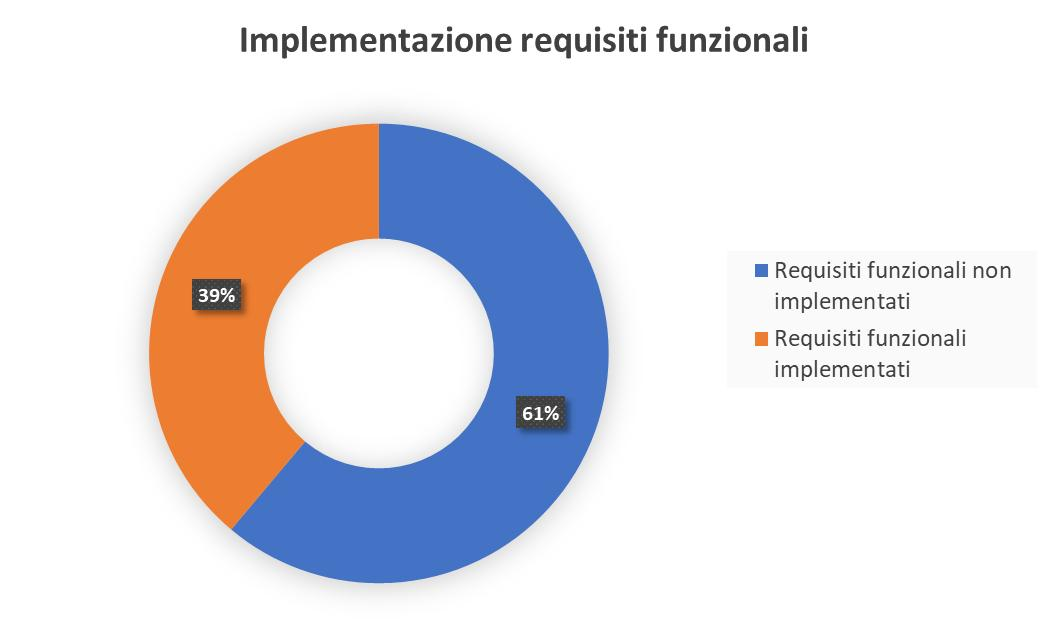
\includegraphics[width=\textwidth,height=\textheight,keepaspectratio]{./img/Grafici/implementazione_requisiti_funzionali.jpg}
            \caption{Grafico implementazione requisiti funzionali}
        \end{figure}
        \begin{figure}[H]
            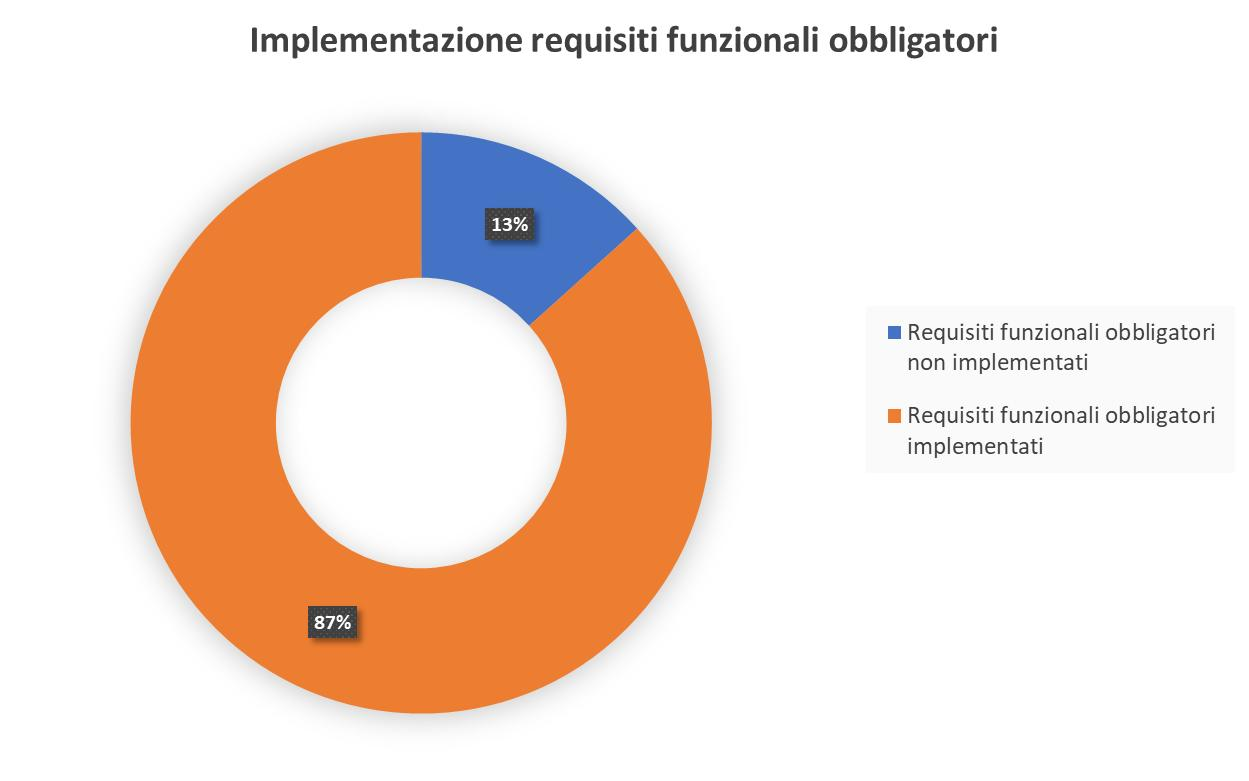
\includegraphics[width=\textwidth,height=\textheight,keepaspectratio]{./img/Grafici/implementazione_requisiti_funzionali_obbligatori.jpg}
            \caption{Grafico implementazione requisiti funzionali obbligatori}
        \end{figure}
    \subsection{Tracciamento requisiti qualitativi}
        \rowcolors{2}{gray!25}{gray!15}
        \begin{longtable} {
            >{\centering}p{64.5mm} 
            >{}p{64.5mm}
            }
        \rowcolor{gray!50}
            \textbf{Requisito} & \textbf{Implementazione} \TBstrut \\
            R1Q1 & Implementato \TBstrut \\ [2mm]
            R1Q2 & Implementato \TBstrut \\ [2mm]
            R1Q10 & Implementato \TBstrut \\ [2mm]
            R1Q3 & Implementato \TBstrut \\ [2mm]
            R1Q4 & Implementato \TBstrut \\ [2mm]
            R1Q5 & Implementato \TBstrut \\ [2mm]
            R2Q6 & Implementato \TBstrut \\ [2mm]
            R1Q7 & Implementato \TBstrut \\ [2mm]
            R1Q8 & Implementato \TBstrut \\ [2mm]
            R1Q9 & Implementato \TBstrut \\ [2mm]
            R1Q11 & Implementato \TBstrut \\ [2mm]
            \rowcolor{white}
            \caption{Tracciamento implementazione requisiti qualitativi}
        \end{longtable}
        \begin{figure}[H]
            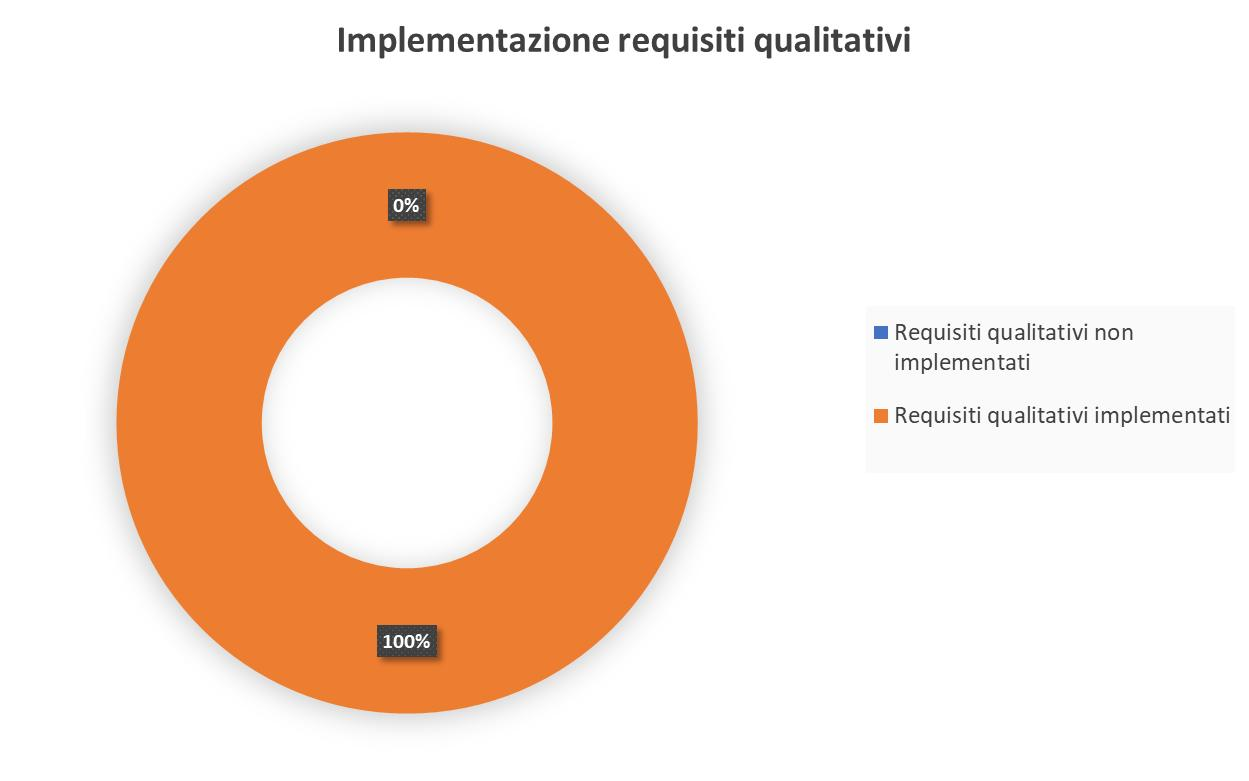
\includegraphics[width=\textwidth,height=\textheight,keepaspectratio]{./img/Grafici/implementazione_requisiti_qualitativi.jpg}
            \caption{Grafico implementazione requisiti qualitativi}
        \end{figure}
        \begin{figure}[H]
            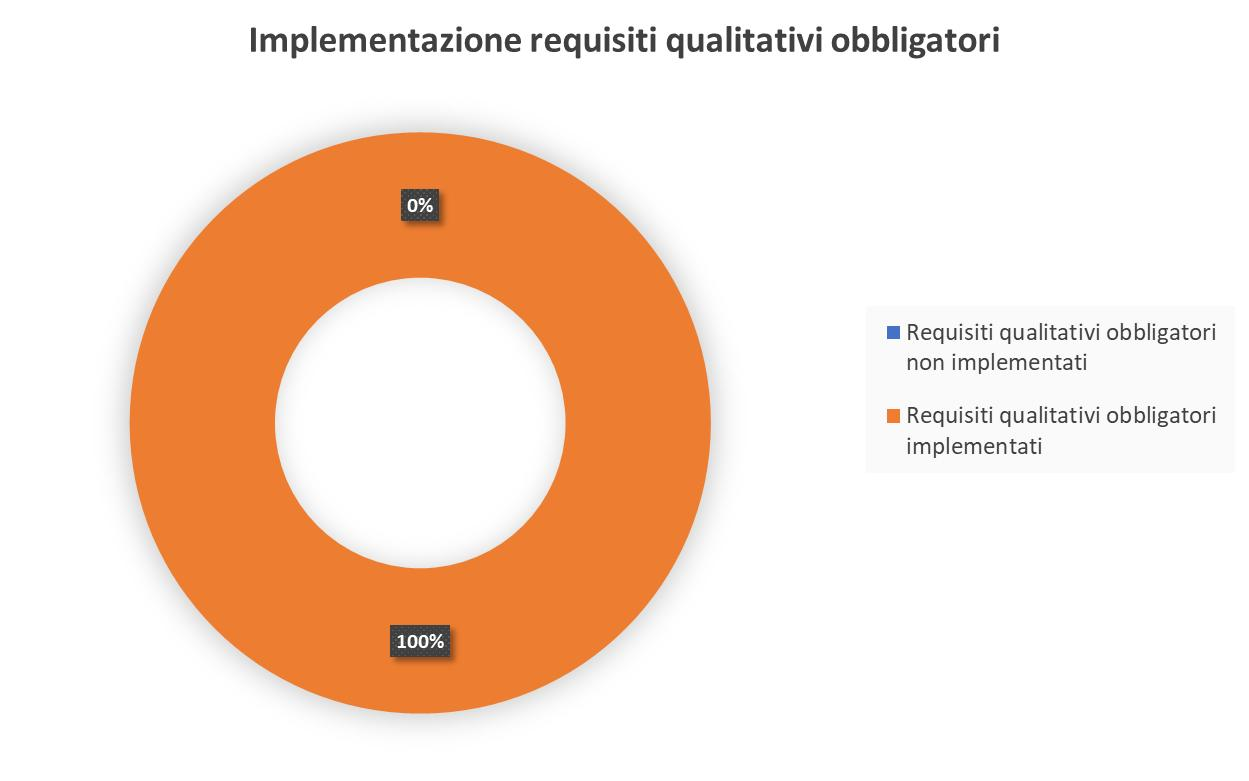
\includegraphics[width=\textwidth,height=\textheight,keepaspectratio]{./img/Grafici/implementazione_requisiti_qualitativi_obbligatori.jpg}
            \caption{Grafico implementazione requisiti qualitativi obbligatori}
        \end{figure}
    \subsection{Tracciamento casi d'uso}
        \rowcolors{2}{gray!25}{gray!15}
        \begin{longtable} {
            >{\centering}p{64.5mm} 
            >{}p{64.5mm}
            }
        \rowcolor{gray!50}
            \textbf{Caso d'uso} & \textbf{Implementazione} \TBstrut \\
            UC1 & Non implementato \TBstrut \\ [2mm]
            UC1.1 & Non implementato \TBstrut \\ [2mm]
            UC1.2 & Non implementato \TBstrut \\ [2mm]
            UC1.3 & Non implementato \TBstrut \\ [2mm]
            UC1.4 & Non implementato \TBstrut \\ [2mm]
            UC1.5 & Non implementato \TBstrut \\ [2mm]
            UC1.6 & Non implementato \TBstrut \\ [2mm]
            UC1.7 & Non implementato \TBstrut \\ [2mm]
            UC1.8 & Non implementato \TBstrut \\ [2mm]
            UC1.9 & Non implementato \TBstrut \\ [2mm]
            UC1.10 & Non implementato \TBstrut \\ [2mm]
            UC1.11 & Non implementato \TBstrut \\ [2mm]
            UC1.12 & Non implementato \TBstrut \\ [2mm]
            UC1.13 & Non implementato \TBstrut \\ [2mm]
            UC1.14 & Non implementato \TBstrut \\ [2mm]
            UC2 & Non implementato \TBstrut \\ [2mm]
            UC2.1 & Non implementato \TBstrut \\ [2mm]
            UC2.2 & Non implementato \TBstrut \\ [2mm]
            UC2.3 & Non implementato \TBstrut \\ [2mm]
            UC3 & Non implementato \TBstrut \\ [2mm]
            UC4 & Implementato \TBstrut \\ [2mm]
            UC4.1 & Implementato\TBstrut \\ [2mm]
            UC4.2 & Implementato \TBstrut \\ [2mm]
            UC4.3 & Implementato \TBstrut \\ [2mm]
            UC4.4 & Implementato \TBstrut \\ [2mm]
            UC4.5 & Implementato \TBstrut \\ [2mm]
            UC4.6 & Implementato \TBstrut \\ [2mm]
            UC4.7 & Implementato \TBstrut \\ [2mm]
            UC4.8 & Implementato \TBstrut \\ [2mm]
            UC4.9 & Implementato \TBstrut \\ [2mm]
            UC4.10 & Implementato \TBstrut \\ [2mm]
            UC4.11 & Implementato \TBstrut \\ [2mm]
            UC4.12 & Non implementato \TBstrut \\ [2mm]
            UC4.13 & Non implementato \TBstrut \\ [2mm]
            UC4.14 & Non implementato \TBstrut \\ [2mm]
            UC4.15 & Non implementato \TBstrut \\ [2mm]
            UC5 & Non implementato \TBstrut \\ [2mm]
            UC5.1 & Non implementato \TBstrut \\ [2mm]
            UC5.2 & Non implementato \TBstrut \\ [2mm]
            UC5.3 & Non implementato \TBstrut \\ [2mm]
            UC6 & Non implementato \TBstrut \\ [2mm]
            UC7 & Implementato \TBstrut \\ [2mm]
            UC8 & Implementato \TBstrut \\ [2mm]
            UC9 & Implementato \TBstrut \\ [2mm]
            UC9.1 & Implementato \TBstrut \\ [2mm]
            UC9.2 & Implementato \TBstrut \\ [2mm]
            UC9.3 & Implementato \TBstrut \\ [2mm]
            UC9.4 & Implementato \TBstrut \\ [2mm]
            UC10 & Non implementato \TBstrut \\ [2mm]
            UC12 & Implementato \TBstrut \\ [2mm]
            UC13 & Non implementato \TBstrut \\ [2mm]
            UC13.2 & Non implementato \TBstrut \\ [2mm]
            UC13.3 & Non implementato \TBstrut \\ [2mm]
            UC13.4 & Non implementato \TBstrut \\ [2mm]
            UC14 & Non implementato \TBstrut \\ [2mm]
            UC15 & Non implementato \TBstrut \\ [2mm]
            UC16 & Non implementato \TBstrut \\ [2mm]
            UC17 & Non implementato \TBstrut \\ [2mm]
            UC18 & Non implementato \TBstrut \\ [2mm]
            UC19 & Implementato \TBstrut \\ [2mm]
            UC20 & Implementato \TBstrut \\ [2mm]
            UC21 & Implementato \TBstrut \\ [2mm]
            \rowcolor{white}
            \caption{Tracciamento implementazione casi d'uso\glo}
        \end{longtable}
        \begin{figure}[H]
            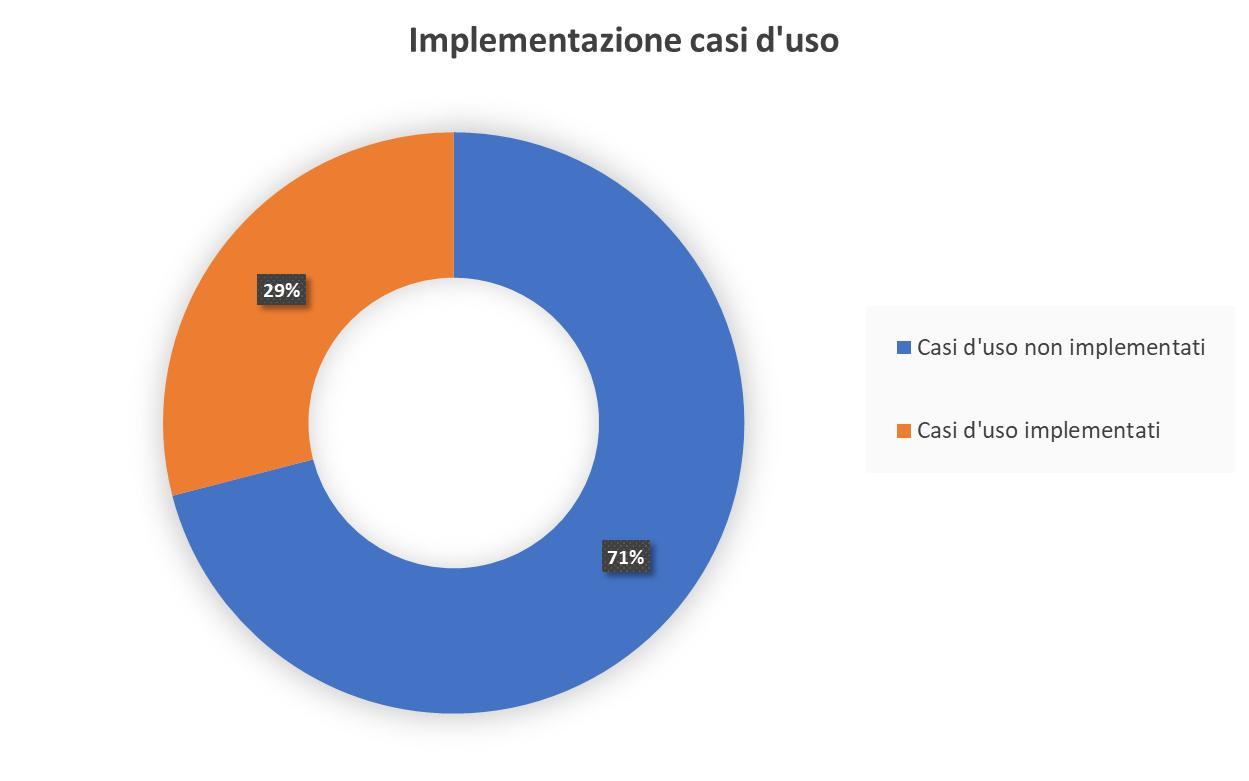
\includegraphics[width=\textwidth,height=\textheight,keepaspectratio]{./img/Grafici/implementazione_casi_d'uso.jpg}
            \caption{Grafico implementazione casi d'uso\glo}
        \end{figure}
	\pagebreak
	
	
	%Input del file "decision_table" della cartella locale "res/"
	%% \textbf = grassetto; \Large = font più grande
% \rowcolors{quanti colori alternare}{colore numero riga pari}{colore numero riga dispari}: colori alternati per riga
% \rowcolor{color}: cambia colore di una riga
% p{larghezza colonna}: p è un tipo di colonna di testo verticalmente allineata sopra, ci sarebbe anche m che è centrata a metà ma non è precisa per questo utilizzo TBStrut; la sintassi >{\centering} indica che il contenuto della colonna dovrà essere centrato
% \TBstrut fa parte di alcuni comandi che ho inserito in config.tex che permetto di aggiungere un po' di padding al testo
% \\ [2mm] : questra scrittura indica che lo spazio dopo una break line deve essere di 2mm

%\setcounter{secnumdepth}{0}
%\hfill \break
%\textbf{\Large{Diario delle modifiche}} \\
\section{Riepilogo tracciamenti}
\rowcolors{2}{gray!25}{gray!15}
\begin{longtable} {
		>{\centering}p{17mm} 
		%>{\centering}p{19.5mm}
		%>{\centering}p{24mm} 
		%>{\centering}p{24mm} 
		>{}p{120mm}}
	\rowcolor{gray!50}
	\textbf{Codice} & \multicolumn{1}{c}{\textbf{Decisione}} \\%\textbf{Decisione} \\ %\TBstrut \\
	VI\_2.1 & Divisione dei ruoli per inizio stesura documenti. \TBstrut \\ [2mm]
	VI\_2.2 & Studio preliminare e divisione del carico di lavoro per le \textit{Norme di Progetto v. 1.1.1} \TBstrut \\ [2mm]
	VI\_2.3 & Stesura domande per l'incontro con il proponente \textit{Zucchetti}. \TBstrut \\ [2mm]
	
\end{longtable} %Tabella delle decisioni (solo per i verbali)
\end{document}